%\documentclassreport]{jsbook}
\documentclass[report, 11pt]{jsbook}
\usepackage[dvipdfmx]{graphicx}
\usepackage{okumacro}
\usepackage{ascmac}
\usepackage{url}
%\usepackage{listings,jlisting}
\usepackage{listings}%,jlisting}
\usepackage{slashbox}

\lstset{
    language=Java,
    basicstyle=\ttfamily\scriptsize,
    commentstyle=\textit,
    classoffset=1,
    keywordstyle=\bfseries,
    frameround=tttt,
    frame=single,
    framesep=5pt,
    showstringspaces=false,
    %numbers=left,
    breaklines=true,
    stepnumber=1,
    numberstyle=\scriptsize,
    tabsize=2,
    xrightmargin=0zw,
    xleftmargin=0zw,
}


\setcounter{tocdepth}{2}

\setcounter{secnumdepth}{5}
\makeatletter
\newcommand{\subsubsubsection}{\@startsection{paragraph}{4}{\z@}%
    {1.5\baselineskip \@plus.5\dp0 \@minus.2\dp0}%
    {.5\baselineskip \@plus2.3\dp0}%
    {\reset@font\normalsize\bfseries}
}
\newcommand{\subsubsubsubsection}{\@startsection{subparagraph}{5}{\z@}%
    {1.5\baselineskip \@plus.5\dp0 \@minus.2\dp0}%
    {.5\baselineskip \@plus2.3\dp0}%
    {\reset@font\normalsize\itshape}
}
\makeatother
\setcounter{tocdepth}{5}

\begin{document}

\pagestyle{empty}

\begin{center}

\vspace{5cm}

\textbf{\Large 卒業論文2014年度(平成26年度)}

\vspace{1cm}

\textbf{\LARGE T-Ring:センサデータの時間的特殊性に着目した多次元データ分散管理システム}
\vspace{3cm}

\textbf{\underline{\large 指導教員}}\\
\textbf{慶應義塾大学環境情報学部}

\textbf{\Large 徳田 英幸}\\
\textbf{\Large 村井 純}\\
\textbf{\Large 楠本 博之}\\
\textbf{\Large 中村 修}\\
\textbf{\Large 高汐 一紀}\\
\textbf{\Large Rodney D. Van Meter III}\\
\textbf{\Large 植原 啓介}\\
\textbf{\Large 三次 仁}\\
\textbf{\Large 中澤 仁}\\
\textbf{\Large 武田 圭史}

\vspace{6cm}

\textbf{\LARGE 慶應義塾大学 環境情報学部}

\vspace{.5em}

\textbf{\LARGE 小町 芳樹}

\vspace{.3em}

\textbf{\it ysk@ht.sfc.keio.ac.jp}



\newpage

\end{center}

\pagestyle{plain}


\frontmatter
\begin{center}
\textbf{\Large 卒業論文要旨 2014年度(平成26年度)}

\vspace{6.18mm}

\textbf{\Large T-Ring:センサデータの時間的特殊性に着目した多次元データ分散管理システム}
\end{center}

\vspace{10mm}
近年,センサネットワークは環境モニタリングや,スマートグリッドなど,我々の生活を豊かにするインフラとして整備されつつある.また,センサノードの小型化やセンサを搭載したスマートフォンの普及により,センサ自体やセンサネットワークが,家庭,個人の規模で利用されつつあり,センサネットワークが我々を支える生活基盤と成り得る将来は遠くはない.

本研究は,センサネットワークがより一般的な生活基盤となり,他の組織や家庭などとデータを公開,共有し,センサの具体的な所在を気にすることなく,自由にデータを利用できる世の中を想定する.この環境下で,公開,共有されたセンサデータを公衆センサデータとする.

この公衆センサデータの管理を行うには,センサデータを緯度,経度,センサタイプを含んだ多次元のデータとして扱わなければならないが,従来の多次元データ管理の研究において,センサデータを対象とした研究は数が多くない.また,センサデータを対象にしていても,センサデータの時間的特殊性という性質に着目している研究は存在しない.

本研究は,このセンサデータの時間的特殊性に着目した多次元データ管理システムであるT-Ringを提案する.T-Ringは時間を多次元データにおける1つの属性とせず,保存先変更の基準として扱うことで,データの保存,取得時の計算量を減らし,処理時間を減少させる.さらに,本研究ではこのT-Ringシステムの性能を評価することで,有用性を証明する.

\vspace{10mm}
キーワード :\\
\hspace{3.5em}公衆センサデータ, 多次元データ管理,P2P,分散ネットワーク,構造化オーバーレイネットワーク

\begin{flushright}
\textbf{慶応義塾大学環境情報学部}\\
\textbf{小町芳樹}
\end{flushright}

\newpage

\begin{center}
\textbf{\Large Abstract of Bachelor's Thesis}
\textbf{\Large Academic Year 2014}
\vspace{6.18mm}

\textbf{\Large T-Ring:Sensor Data Oriented Decentralized Multidimensional Indexing Focusing on Particularity of Time}
\end{center}

\vspace{10mm}

In recent years, sensor networks are being developed as an infrastructure to enrich our lives such as environmental monitoring and smart grids. In addition, by the spread of sensor equipped smartphones and downsizing of sensor nodes, sensor networks (or the sensor itself) are being used in the scale of family or personal. In the future, sensor networks will become the foundation of our life supporting. 

This research assumes that sensor networks could become the foundation and that everyone could get data from anywhere without being concerned about which sensor network they belong to. In this environment, these published and shared sensor data are called "public sensor data" in this paper. 

To manage this public sensor data, sensor data should be operated as Multidimensional Indexing which has latitude, longitude, sensor type and so on. However, in general works of Multidimensional Indexing, these researches were hardly intended on sensor data. No reserach focused on particularity of sensor time.   


This research proposes T-Ring which is Multidimensional Indexing system for public sensor data. This is the first research focusing on particularity of sensor time. T-Ring doesn't use time attributtion in multidimensional data and  use a criterion of deciding the place of storage. T-Ring reduces amount of calculations on storing and retrieving of data and processing speed. This paper evaluates this system and proves feasibility.   

\vspace{10mm}
Keywords :\\
\hspace{3.5em}Public Sensor Data, Multidimensional Indexing, P2P, Decentralize Network, Structured Overlay Network
\begin{flushright}
\textbf{Yoshiki Komachi}\\
\vspace{5mm}
\textbf{Faculty of Environment and Information Studies}\\
\textbf{Keio University}
\end{flushright}

\tableofcontents
\listoffigures
\listoftables

\mainmatter
\chapter{序論}
\begin{large}
\begin{quote}
本章では,まずセンサデータの増加などの本研究の背景を述べ,次いで,センサデータの公衆一般化において発生する問題の解決という本研究の目的について言及し,最後に本論文の構成を示す.
\end{quote}
\end{large}
\clearpage

\section{本研究の背景}
近年センサの低価格化,高性能化により,センサネットワークが普及し,
それに伴いセンサ用のオペレーティングシステムの研究も発展を遂げている.
センサネットワークのオペレーティングシステムには主に2種類あり,
省資源性かつ低オーバヘッドを実現したイベントモデルと,
リアルタイム処理を可能としたマルチスレッドモデルが存在している.
センサネットワーク用のオペレーティングシステムではイベントモデルが主流となっている.

イベント駆動型のTinyOSは,省資源かつ低オーバヘッドの実現に成功しているが,
リアルタイム処理を行うことができていない.
また,言語もnesCという特殊な言語を使用しているため,
プログラムが非常に書きにくいという欠点も存在する.
それに対して,Nano-RKはリアルタイム処理をサポートしているが,
イベント駆動型のオペレーティングシステムと比較すると資源の消費が大きく,
高オーバヘッドである.

Contikiはイベント駆動型のオペレーティングシステムで,使用言語はC言語である.
ContikiはProtothreadsと呼ばれるメカニズムを使用しており,
イベント駆動型でありながらスレッドの切り替えを行うことができる.
そのため,イベント駆動型の特徴となっているプログラムの書きにくさを解消することに成功している.
しかし,タスクを処理する優先順位を明確に決める手法が定められていないため,
タスクの切り替えはできるが,未だにリアルタイム処理は不可能なのが現状である.


\section{本研究の目的}
Contikiはイベント駆動型でありながら,
マルチスレッドでタスクを変更することができるため,
リアルタイム処理と親和性があると推測できる.
本研究では,Contikiにスケジューラを実装し,
省資源性かつ低オーバヘッドでありながら,
リアルタイム処理の可能なオペレーティングシステムの実現を目的とする.
最後に,本システムの評価を行うとともに,有用性を証明する.


%多次元データに対して,センサデータの時間的特殊性を考慮した,T-Ringという分散管理手法を提案し,管理について,利用するアプリケーションの特徴を幾つかの軸で分類し,既存の手法を用いたシステムがどのようなアプリケーションに適するのかを明らかにする.次に,センサデータの時間的特殊性を考慮したシステムが必要なアプリケーションを提示する.最後に,センサデータの時間的特殊性を考慮したシステムの提案し,パフォーマンスの低下を防ぐ.

\section{本論文の構成}
本論文では,2章において,センサネットワークの一般公衆化とアプリケーションの分類から,そのデータ管理において必要な機能要件を示し,センサデータの時間的特殊性について述べる.3章では,センサデータではない公衆コンテンツの管理とDHTを用いた広域公衆センサデータについての関連研究を紹介する.4章,5章では,センサデータの時間的特殊性に着目したデータ管理システムを示す.6章で,提案手法に対する評価を行い,7章で本研究のまとめを行う.

\chapter{無線センサネットワーク}
\begin{large}
\begin{quote}
本節では,最初に多次元データ管理Multidimensional Indexing(MI)の分野における関連研究を挙げる.次に,Contents Delivery Network(CDN)におけるコンテンツの特徴を利用したレプリケーションを行った研究を挙げる.最後に,センサデータを多次元データとして扱った研究を挙げる.
\end{quote}
\end{large}
\clearpage

\section{はじめに}


\section{イベント検知アプリケーション}
\begin{figure}[htbp]
 \begin{center}
  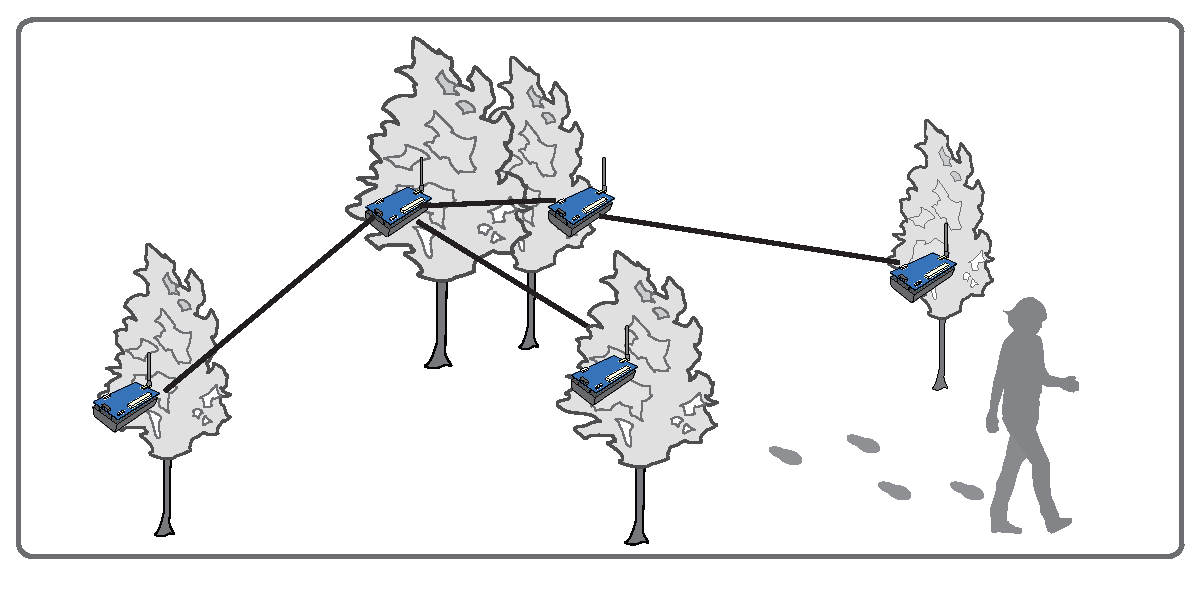
\includegraphics[width=100mm]{./images/event_detection.eps}
 \end{center}
 \caption{イベント検知アプリケーション}
 \label{fig:event_detection}
\end{figure}


%\section{多次元データ管理}
%1990年代から,データベースの分野において,多次元のデータをどのように管理するべきかMultidimensional Indexing(MI)\cite{Gaede:1998:MAM:280277.280279}が議論されている.そして,地理学,ロボット工学,環境保護学などの様々な分野でこのMIは応用されている.1990年代のMIの中心はデータが集中管理されている環境を想定したアルゴリズムであり,VA\_File\cite{Weber:1998:QAP:645924.671192},Hilbert R-tree\cite{Kamel:1994:HRI:645920.673001},GHT\cite{Ratnasamy:2002:GGH:570738.570750}などがその代表である.2000年代からは,P2Pを用いた分散型のMIが主流となる.2000年代前半に提案されたChord\cite{Stoica:2001:CSP:383059.383071},CAN\cite{Ratnasamy:2001:SCN:383059.383072},SkipGraph\cite{Aspnes:2003:SG:644108.644170}が代表である.2000年代後半から現在にいたるまでにこれ以外の数多くのアルゴリズムが提案されているが,大半がこのいずれかのアルゴリズムの変形であって,大きなアルゴリズムの変化はない.
%
%センサデータが公衆化し,広域に管理される場合,2.2節で述べられているように,データの値以外のインデックスが付与される必要がある.よって,公衆広域センサデータを多次元データとして管理しなければならない.
%\begin{figure}[htbp]
% \begin{center}
%  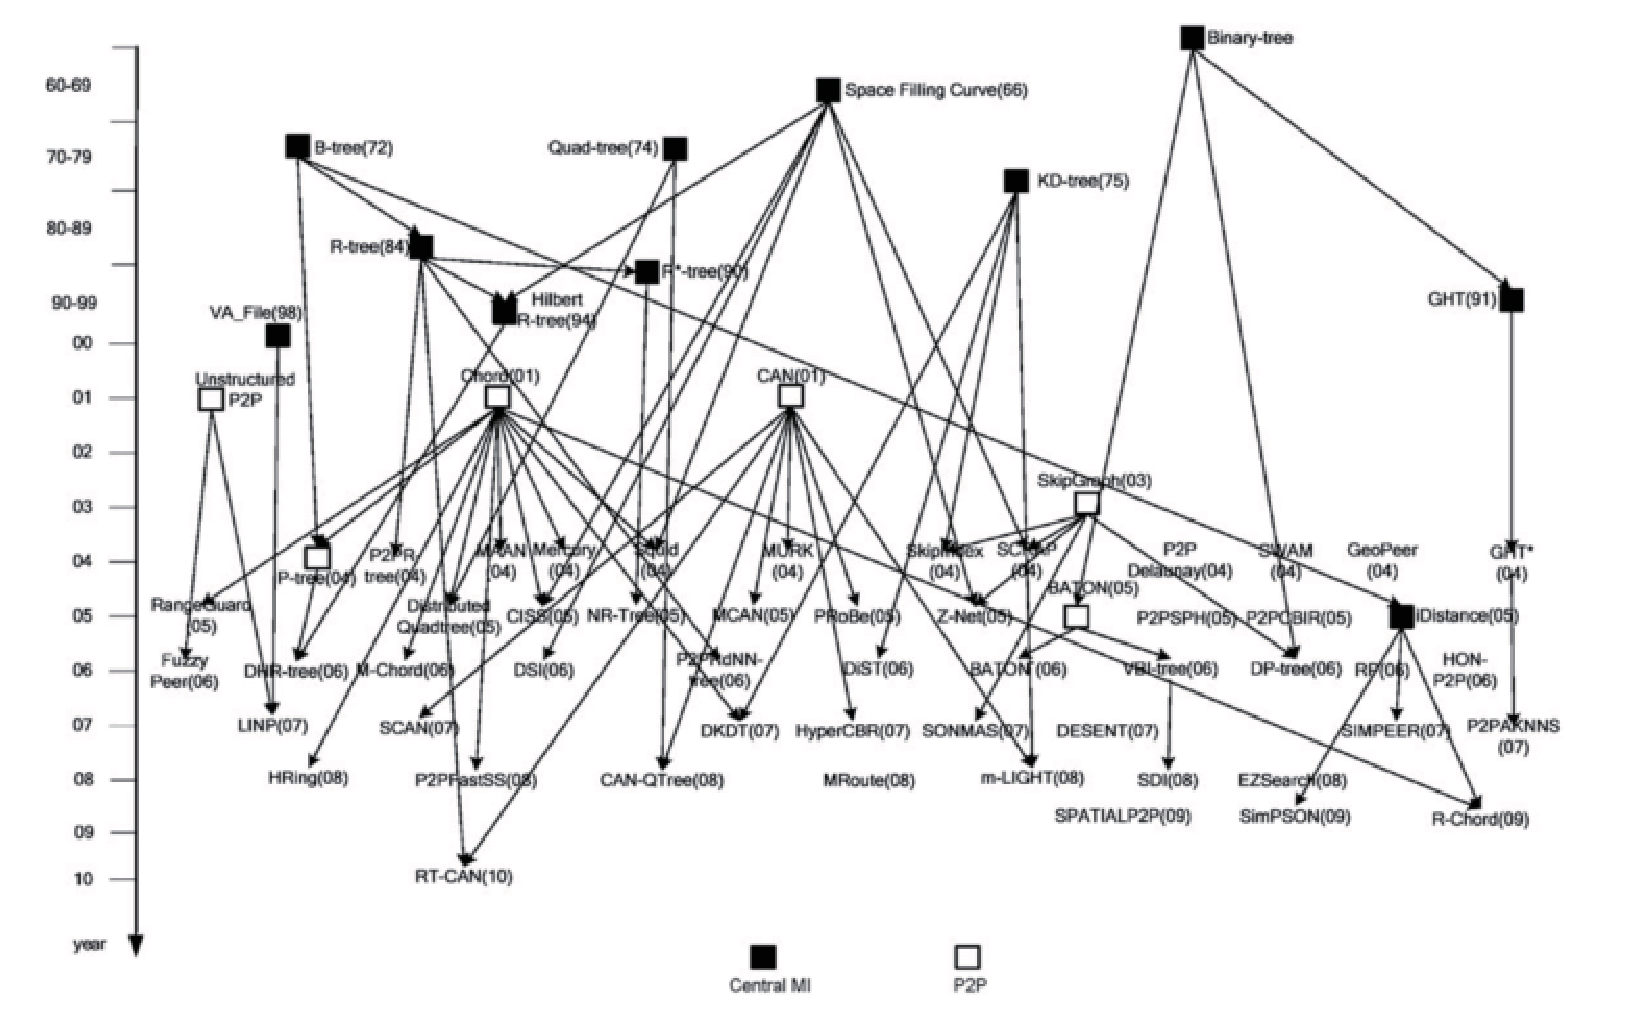
\includegraphics[width=130mm]{./images/MI_history.eps}
% \end{center}
% \caption{Multidimensional Indexingの歴史(参考:P2P-based multidimensional indexing methods. Journal of Systems and Software 2011\cite{Zhang:2011:PMI:2039458.2039840})}
% \label{fig:MI_history}
%\end{figure}
%
%
%
%\section{文書や音楽などのコンテンツの広域管理}
%この多次元データ管理は,Akamai\cite{Akamai}などに代表される,Contents Delivery Network(CDN)などで利用されている.CDNは世界中の数十,数百のデータセンターでP2Pネットワークを構築し,ユーザーに音楽や動画などを提供している.コンテンツには,サイズ,言語などの多次元のインデックスが付与されている.CDNは,コンテンツの特徴を抽出し,レプリケーション先を決定し,効率的なコンテンツの配送を実現している.Chaら\cite{Cha:2009:MAI:1526709.1526806}は,Flickr\cite{Flickr}のコンテンツがどのように伝播するのかの調査をしている.Scellatoら\cite{Scellato:2011:TGD:1963405.1963471}はtwitter\cite{twitter}やfacebook\cite{Facebook}などのSNSなどに載せられたコンテンツとその発言などのいち情報から,コンテンツの地域性を割り出し,レプリケーションを効率的に行う手法を提案している.Akamaiでは,トラフィックの状況などを公開しており,時間帯や地域による傾向を捉えることができる.関連研究ではコンテンツの言語から地域性を抽出し,対象地域のデータセンターに予めコンテンツをレプリケーションすることにより,効率化を実現している.この他にも,コンテンツや利用状況の特徴を抽出するために\cite{Tang:2012:MAA:2310257.2310450}\cite{Labovitz:2010:IIT:1851182.1851194}\cite{Maier:2009:DCR:1644893.1644904}\cite{Otto:2011:BME:2018436.2018450}などのインターネット計測の分野の研究結果も利用されている.
%
%\begin{figure}[htbp]
% \begin{center}
%  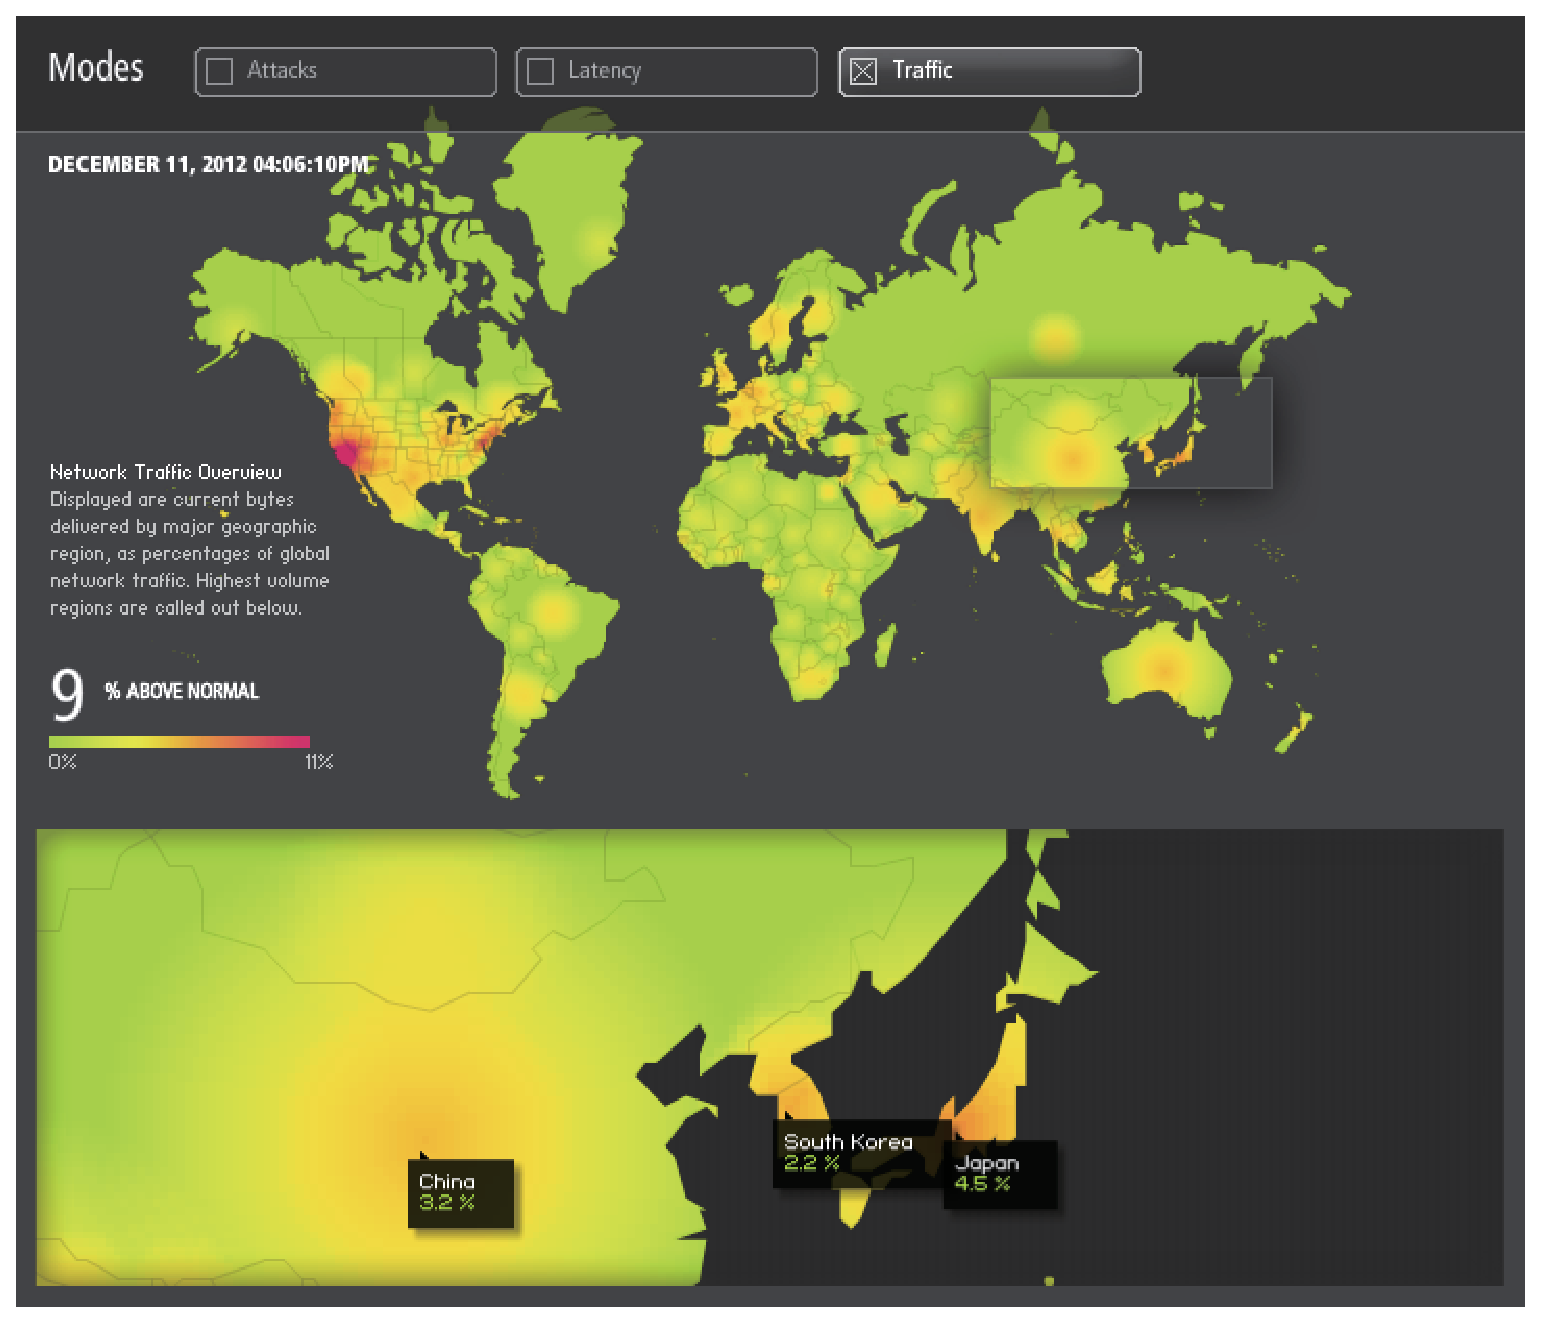
\includegraphics[width=100mm]{./images/akamai.eps}
% \end{center}
% \caption{Akamaiによるトラフィック情報の公開(参考:Akamai\cite{Akamai})}
% \label{fig:akamai}
%\end{figure}
%
%センサデータは2.3節で取り上げた,音楽や動画とは異なる時間的特殊性に加え,言語などから由来する地域性も存在しないため,コンテンツの特徴からレプリケーションの場所を決定するという手法を取ることができない.
%
%\section{DHTを用いた公衆センサデータ管理}
%広域センサデータを多次元データとして,MIのアルゴリズムを用いた研究にSynapse\cite{Terayama:2012:DSD:2370216.2370335}がある.この研究では,従来の,発せられたセンサデータを地理的に近い保存ストレージに保存するという手法では,イベントの発生による突発的な人口過密が発生した際に,特定のセンサデータ保存ストレージに対する保存,取得のクエリが集中すると主張している.そこで,センサデータの緯度,経度,センサタイプ,データの時間を空間充填曲線\cite{Lawder:2000:USC:646102.681186}図\ref{fig:zorder}を用いて1次元化する.空間充填曲線はLawderらが提案した,DHTアルゴリズムにおいて,多次元データを1次元化する手法で,これにより多次元データをハッシュ関数にかけることが可能になる.この手法はMIにおける基本的な手法であり,2009年にKantereらが提案したSPACIALP2P\cite{Kantere:2009:SIS:1495799.1496017}というMIアルゴリズムでも用いられている.このハッシュ化した値を元にDHTネットワークを構築することで,特定の保存ストレージに対するクエリの集中を防いでいる.
%
%しかし,Synapseではセンサデータの時間的特殊性が考慮されていないため,利用状況によっては,パフォーマンスが低下してしまう可能性がある.
%\begin{figure}[htbp]
% \begin{center}
%  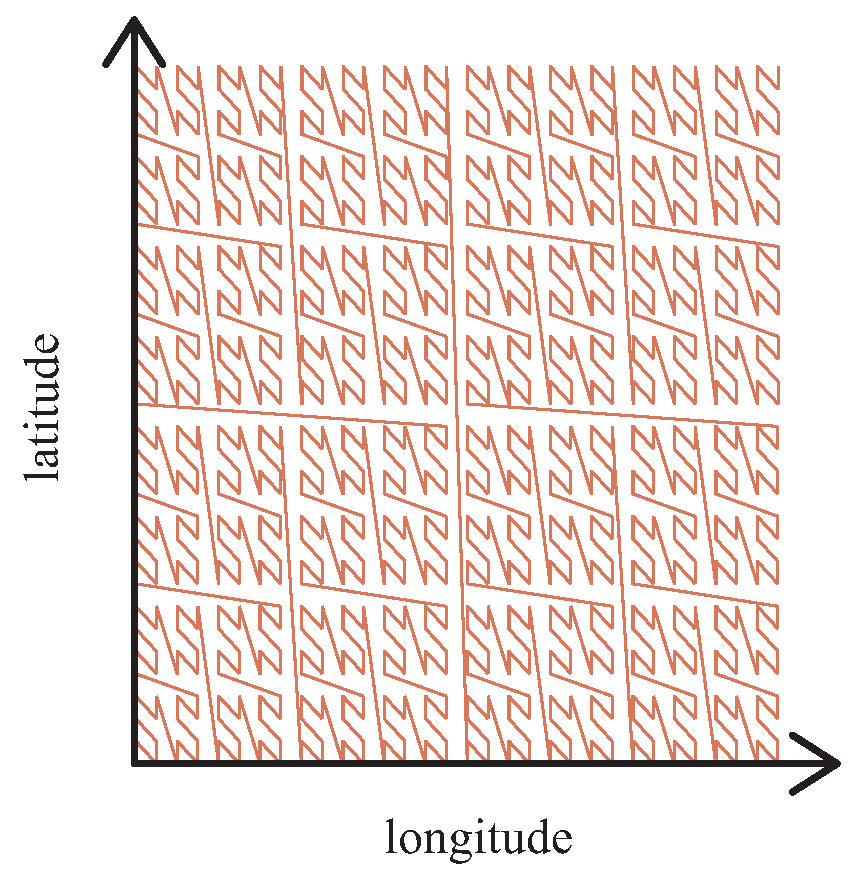
\includegraphics[height=100mm]{./images/zorder.eps}
% \end{center}
% \caption{空間充填曲線:Z-order}
% \label{fig:zorder}
%\end{figure}



\section{まとめ}
本章では,まず,公衆広域センサデータが多次元データであるということから,本研究の根幹を成す,Multidimensional Indexing(MI)という研究分野を紹介した.次に,Contents Delivery Network(CDN)という分散したデータセンターで多次元データを管理するネットワークという観点から捉え,センサデータにはCDNで扱われるような特殊性が存在しないことを述べた.最後に,公衆広域センサデータの分散管理手法を紹介し,センサデータの時間的特殊性が考慮されていないことに言及した.

\chapter{無線センサネットワークにおけるオペレーティングシステム}
\begin{large}
\begin{quote}
本章では,最初にセンサネットワークの一般公衆化を説明し,公衆センサデータ管理における必須な機能要件である地理的探索について述べる.次に,公衆センサデータ管理のシステム設計の際の重要な概念であるデータ管理の時間的密度を解説し,最後にセンサデータの時間的特殊性とそれに起因する公衆センサデータ管理の問題点を述べる.
%本章では、
\end{quote}
\end{large}
\clearpage


%\section{無線センサネットワークにおけるオペレーティングシステム}
%無線センサネットワークのオペレーティングシステムには主に2種類あり、
%イベントモデルとスレッドモデルが存在している。
%無線センサネットワーク用のオペレーティングシステムではイベントモデルが主流となっている。

\section{イベントモデル}
イベントモデルで構築されたオペレーティングシステムは全てのタスクをイベントによって起動し,
run-to-completion で実行する形態のオペレーティングシステムである.
%イベントモデルの動作を図 4 に示す.
イベントモデルはひとつのイベントループと多数のイベントハンドラから構成される.
イベントループはイベントの到着を待ち,
イベントが届くとイベントに関連付けられているイベントハンドラを実行する.
イベントモデルではイベント駆動型プログラミングによってアプリケーションが記述される.
イベントハンドラは寿命の短いrun-to-completionで記述され,
プリエンプションされることがない.
つまり,イベントモデルはタスクは関数呼び出しと等価であり,
実行ストリームがひとつで実現されるため各タスクでローカル変数の領域を共有可能なので
省資源かつ低オーバヘッドで並列性を実現できる.
また,各タスクが不可分に実行されるので共有資源に対する排他制御が不要となり,
安全性が高い.
さらに,CPU の特殊な機能を用いなくても実装できるので移植性も高い.
\begin{figure}[htbp]
 \begin{center}
  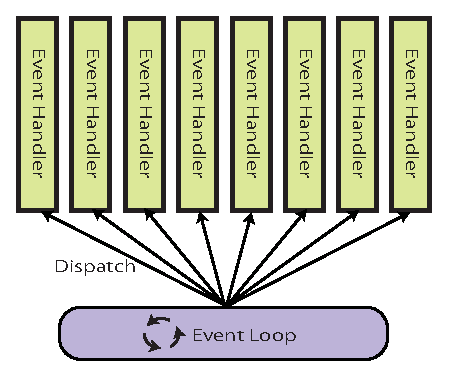
\includegraphics[width=60mm]{./images/event_model.eps}
 \end{center}
 \caption{イベントモデル}
 \label{fig:event_model}
\end{figure}


%\subsection{TinyOS: An Operating System for Sensor Networks}
\subsection{TinyOS}
この中で代表的なものがTinyOS\cite{Hill:2000:SAD:356989.356998}\cite{Levis04tinyos:an}である.
TinyOSはカリフォルニア大学バークレー校のSmartDust Projectで開発されたオペレーティングシステムである.
現在無線センサネットワークの標準的なオペレーティングシステムとして扱われており,
Crossbow社から発売されているMICA2やMICAz\cite{Hill:2002:MWP:623308.624560},
Telos\cite{Polastre:2005:TEU:1147685.1147744},iMote\cite{Nachman:2005:IMP:1147685.1147760}上で動作する.
TinyOSはCPUの特別な機能を使用せずに実装可能であるため,移植性が高く,
ATMELのAVR128LやTexsusのMSP430,ARM7などさまざまなCPUに移植されている.

TinyOSではnesC\cite{Gay:2003:NLH:781131.781133}と呼ばれるイベント駆動型の新しい言語で
複数のイベントハンドラを 1 つのモジュールとして設計可能な機能を提供することで
イベントモデルの持つプログラムの開発のし辛さを提供している.
さらに,nesCはイベント駆動型に特化した最適化を行っているので省資源性も実現される.


%\subsection{A Dynamic Operating System for Sensor Nodes}
\subsection{SOS}


\section{スレッドモデル}
%スレッドモデルを図 5 に示す.
スレッドモデルは複数のスレッドから構成される.
各スレッドはそれぞれ独立に実行ストリームを持っており,
低い優先度のスレッドは高い優先度のスレッドにプリエンプションされるという特徴を持つ.
スレッドモデルではユーザはあたかもCPUを占有しているかのように
一連の処理をひとつのスレッドとして記述することができるので
プログラムが書きやすい.
また,プリエンプションを行うことも想定しているので
ハードリアルタイム処理をサポートすることができる.
\begin{figure}[htbp]
 \begin{center}
  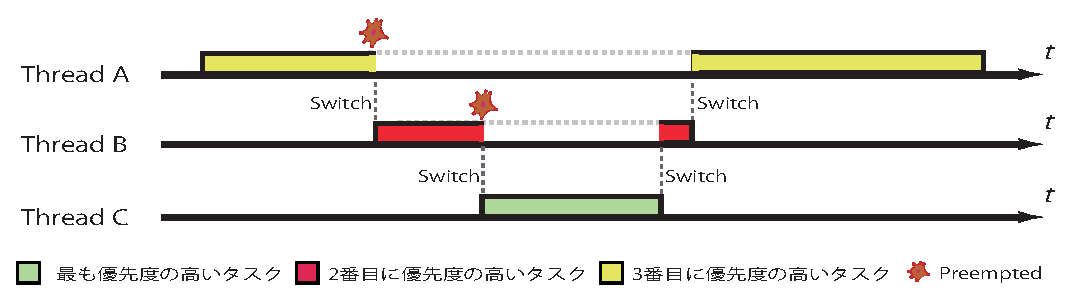
\includegraphics[width=140mm]{./images/threads_model.eps}
 \end{center}
 \caption{スレッドモデル}
 \label{fig:threads_model}
\end{figure}


%\subsection{Nano-RK: an Energy-aware Resource-centric RTOS for Sensor Networks}
\subsection{Nano-RK}



%\subsection{MANTIS OS: An Embedded Multithreaded Operating System for Wireless Micro Sensor Platforms}
\subsection{MANTIS OS}


%ジョブの実行を設定された時間通りに作動させることをリアルタイム処理という.
%リアルタイム処理には主に
%ハードリアルタイム処理と
%ソフトリアルタイム処理,の2種類がある.
%
%
%\subsection{ハードリアルタイム処理}
%課せられた処理が期限内に終了しなかったとき,
%システム全体に致命的なダメージが生じてしまうリアルタイム処理のことを
%ハードリアルタイム処理という.
%したがって,期限内での終了が保証されなければならないシステムに用いられる.
%
%\subsection{ソフトリアルタイム処理}
%ソフトリアルタイム処理を行うシステムでは,
%期限内に処理が終了しなくてもシステム全体に致命的なダメージを与えることはない.
%ただし,処理自体の価値は終了期限とともに減少していく.


\section{イベントモデルとスレッドモデルの比較}
しかしながら,
ユーザが一連の処理を細かい処理に分割しなければならないのでプログラムが書き辛いという問題が発生する.

さらに,イベントモデルではタスクのプリエンプションをしないことを前提に設計されているので
ハードリアルタイム処理のサポートができない.
しかしながら,プリエンプション時のオーバヘッドの大きいことや必要とされる資源が多いこと,
スレッド間の共有資源へのアクセス制御が必要となるために安全性が損なわれるなどの問題を持っている.

\begin{table}[htb]
  \centering
  \caption{オペレーティングシステムの比較}
  \begin{tabular}{|c||c|c|c|c|} \hline
    \backslashbox{}{} & \multicolumn{2}{|c|}{メリット} & \multicolumn{2}{|c|}{デメリット} \\ \hline \hline
    イベントモデル & 省資源 & 低オーバヘッド & リアルタイム性の非サポート & プログラムが記述しにくい \\ \hline
    スレッドモデル & \multicolumn{2}{|c|}{リアルタイム性のサポート} & 資源の消費が大きい & 高オーバヘッド \\ \hline
  \end{tabular}
  \label{tab:merit_and_demerit}
\end{table}

\section{まとめ}
本章では,まず,センサネットワークの一般公衆化について述べた.次いで,公衆センサデータがを扱ったシステム設計をする際に,データ管理の時間的密度という要素を考慮すべきであることを示した.そして,センサデータが時間的特殊性を持った多次元データであることを述べ,また,それに起因するセンサデータ管理における問題を提起した.
%システムにおける地理的探索の必要性について記した.さらに,センサデータ以外のコンテンツを扱うシステムとセンサデータを扱うシステムの対比を行い,広域センサデータ管理システムにおけるデータ管理の時間的密度という概念を説明し,最後に,センサデータの時間的特殊性を取り上げた後,それに起因するセンサデータ管理におけるデータ管理の時間的密度の高さという問題を提起した.

\chapter{Contiki - a Lightweight and Flexible Operating System for Tiny Networked Sensors}
\begin{large}
\begin{quote}
本章では,最初に,本研究が提案するT-Ringという公衆センサデータ管理システムにおける,時間概念の扱いと,それに伴った保存アルゴリズムの概念説明を行う.次に,集中管理とSynapseとのデータ管理の時間的密度と計算コストの比較を行う.詳細な設計については次章で解説する.

\end{quote}
\end{large}
\clearpage

\section{Protothreads}
既に述べたように,イベント駆動型は組み込みシステムやセンサネットワークに対して,
主流なオペレーティングシステムとなっている.
しかし,イベント駆動型はメモリのオーバヘッド低く維持できる一方で,
ユーザが一連の処理を細かい処理に分割しなければならないため,
プログラムが書き辛いという問題が発生する.
%TinyOSの例
Protothreads\cite{Dunkels:2006:PSE:1182807.1182811}はイベント駆動型プログラムをマルチスレッド型のように記述することができるため,
メモリのオーバヘッドを抑えつつ,
イベント駆動型の欠点を補うことが可能となる.
本節では,Protothreadsの機能について詳しく述べる.

\subsection{メモリ}
マルチスレッド型のオペレーティングシステムでは,
図\ref{fig:threads_stack}のようにそれぞれのスレッドにそれぞれのスタックを必要とする.
しかし,メモリが制限されているセンサネットワークのようなシステムでは,
スタック用のメモリは静的に保持されなければならないため,
このメモリを他の目的で使用することはできない.
\begin{figure}[htbp]
 \begin{center}
  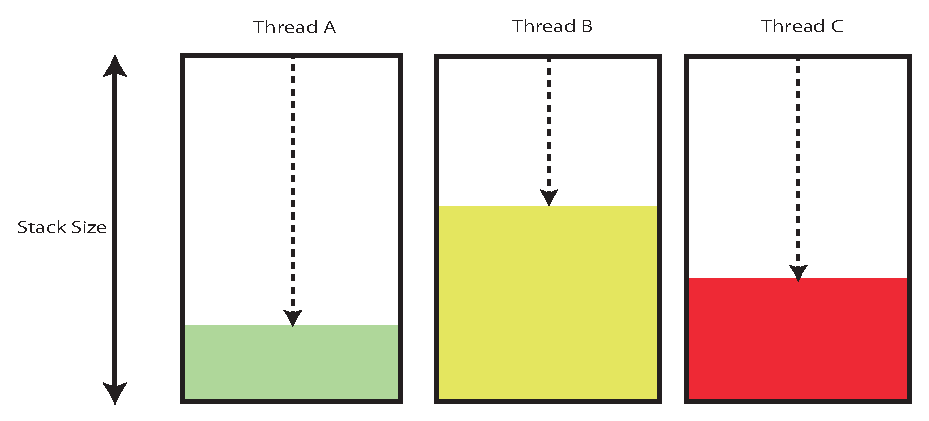
\includegraphics[width=110mm]{./images/threads_stack.eps}
 \end{center}
 \caption{一般的なスレッドモデルにおけるスタック}
 \label{fig:threads_stack}
\end{figure}

それに対して,Protothreadsにおけるスタックを図\ref{fig:protothreads_stack}に示す.
Protothreadsを使用した場合,
すべてのプログラムは同じスタックを共有し,
実行されることとなる.
つまり,Protothreadsを利用しているオペレーティングシステムではそのような事態を防ぐために,
マルチスレッドを実現しつつも,ひとつのスタックをあたかも複数個あるように見せかけている.
\begin{figure}[htbp]
 \begin{center}
  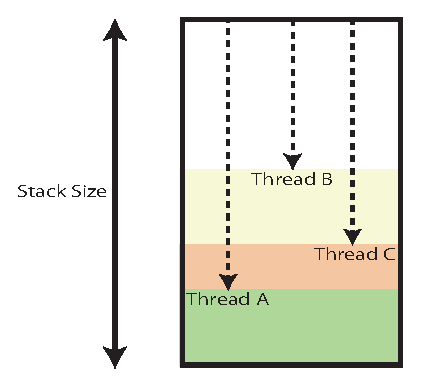
\includegraphics[width=45mm]{./images/protothreads_stack.eps}
 \end{center}
 \caption{Protothreadsにおけるスタック}
 \label{fig:protothreads_stack}
\end{figure}


\subsection{タスクの切り替え}
一般的なマルチスレッド型のオペレーティングシステムは,
タスクの割り込みがあった際には,
レジスタの状態を保存することで変数の値を保持し,
割り込まれたタスクの実行が終了したときに,
再びレジスタから変数を読み込み,
処理を途中から再開する.

しかし,Protothreadsを使用した場合,
状態をレジスタに保存することはせずに,
戻り値を利用することでタスクのCPUの利用を放棄する.
さらに,アプリケーション内の変数は静的な変数を採用しているため,
低オーバヘッドを実現しつつ,一貫性を保っている.

戻り値をもとにしたタスクの切り替えを行う際には,
スケジューラに対してプログラムのファイルの行数をreturnし,
各タスクがCPU利用権限を再度取得したとき,
行数を条件分岐し,前回中断した箇所から実行を再開することとなる.

ただし,現在実行中のタスクよりも優先度の高いタスクが実行待ちになった際に,
他のマルチスレッドのオペレーティングシステムで実現されているように,
ループ内の処理を実行しているタスクに割り込みをし,
タスクを切り替えて実行することはできない.

現在では,タイマー割り込みを目的とした利用をされていない.
タイマーと現在時刻を比較し,
発火時刻を過ぎている場合,タスクを実行待ちのキューへと加える.
タイマーを実行するタスクは他のタスクと同じ優先度で周期的に実行される.

\section{イベント}
イベントモデルであるContikiでは,イベントが発生するとプロセスが実行される.
本節ではContikiで扱われる非同期イベントと同期イベントの違いについて説明する.


\subsection{非同期イベント}
非同期イベントが発生すると,
そのイベントはカーネルのイベントキューに挿入され,
実行時にFirst In First Outで呼び出される.

Asynchronous events are delivered to the receiving process some time after they have been posted.
Between their posting and their delivery, 
the asynchronous events are held on an event queue inside the Contiki kernel.

The events on the event queue are delivered to the receiving process by the kernel.
The kernel loops through the event queue and 
delivers the events to the processes on the queue by invoking the processes.



The receiver of an asynchronous event can either be a specific process, or all running processes.
When the receiver is a specific process, the kernel invokes this process to deliver the event.
When the receiver of an event is set to be all processes in the system,
the kernel sequentially delivers the same event to all processes, 
one after another.

非同期イベントはprocess\_post()関数によってポストされる.
process\_post()関数ははじめにキュー内にイベントのためのメモリ空間があるかどうかを決定するために,
現在のイベントキューのサイズを確認する.
もしメモリに空きがなければ,この関数はエラーを返し,
メモリに空きがあった際には,イベントをキューの最後に挿入する.

%Asynchronous events are posted with the process\_post() function. The internals of the process\_post() function is simple.
%It first checks the size of the current event queue to determine if there is room for the event on the queue.
%If not, the function returns an error.
%If there is room for the event on the queue,
%the function inserts the event at the end of the event queue and returns.

\begin{figure}[htbp]
 \begin{center}
  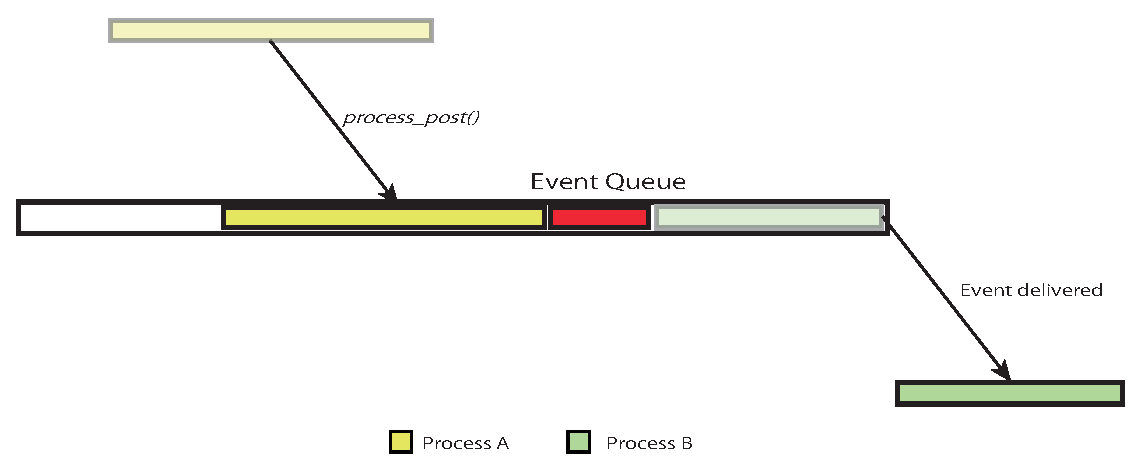
\includegraphics[width=115mm]{./images/fifo.eps}
 \end{center}
 \caption{非同期イベントの実行}
 \label{fig:asynchronous_event}
\end{figure}


\subsection{同期イベント}
When a synchronous event is posted, the event is immediately delivered to the receiving process.

非同期イベントに対して,
同期イベントはポストされたとき,
同期イベント

Unlike asynchronous events, 
synchronous events are delivered directly when they are posted.
Synchronous events can only be posted to a specific processes.

同期イベントは即座に実行されるため,
同期イベントがポストされることは関数を呼び出すことに等しい.

Because synchronous events are delivered immediately,
posting a synchronous event is functionally equivalent to a function call: 
the process to which the event is delivered is directly invoked, 
and the process that posted the event is blocked until the receiving process has finished processing the event.
The receiving process is, however, not informed whether the event was posted synchronously or asynchronously.
\begin{figure}[htbp]
 \begin{center}
  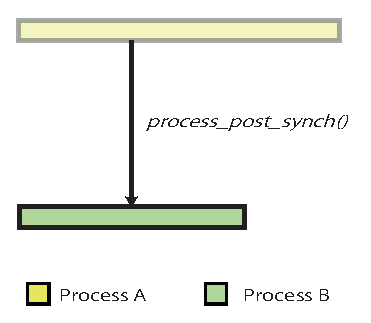
\includegraphics[width=40mm]{./images/synchronous_event.eps}
 \end{center}
 \caption{同期イベントの実行}
 \label{fig:synchronous_event}
\end{figure}


\subsection{ポーリング}
ポーリングリクエストはその他のイベントと異なる
ポールされたプロセスはprocess\_poll()関数によって呼び出され,
この関数がプロセス上で呼び出されるとそのプロセスは可能な限り早急にスケジューリングされる.

A poll request is a special type of event. A process is polled by calling the function process\_poll().
Calling this function on a process causes the process to be scheduled as quickly as possible.
The process is passed a special event that informs the process that it has been polled.

ポーリングはインタラプトからプロセスを実行する手法であり,
process\_poll()関数はプリエンプティブモードから安全に呼び出されるプロセスモジュールにおける,
唯一の関数である.

%Polling is the way to make a process run from an interrupt.
%The process\_poll() function is the only function in the process module that is safe to call from preemptive mode.

\section{イベントタイマー}
Contikiオペレーティングシステムには



\section{問題意識}
イベント駆動モデルではタスクの中断をしないことを前提に設計されているため,
現在のセンサネットワーク用のオペレーティングシステムでは省資源性かつ低オーバヘッドであることと,
リアルタイム性のサポートはトレードオフの関係にある.
しかし,ターゲットトラッキングなどの状況においては,
通常時は省資源性かつ低オーバヘッドを実現し,
イベントが生じた際にはリアルタイム処理を行うことが必要となってくる.
それにも関わらず,現在双方を両立可能としたセンサネットワーク用のオペレーティングシステムは存在していない.

また,Protothreadsが
%イベント駆動型のオペレーティングシステムに実装されていながら,
マルチスレッド型のオペレーティングシステムとの親和性があると推測できることは既に述べたが,
既存のProtothreadsの実装ではイベントに優先度をつけることなく,
First In First Out(FIFO)の要領でイベントを呼び出している(図\ref{fig:asynchronous_event}).
本研究では環境モニタリングやターゲットトラッキングを想定環境としているため,
イベントの到着順でスケジューリングすることは好ましくない.
例えば,優先度の高いタスクが到着したときに既に多量のタスクが実行待ち状態となっている場合に,
高優先度のタスクが実行される頃には,既にそのタスクに実行する価値はない可能性がある.
したがって,既存手法とは別のアルゴリズムを用いてスケジューリングする必要がある.


%前述のとおり,一般的なマルチスレッド型のオペレーティングシステムでは,
%スレッド切り替え時にレジスタの状態を保存するのに対して,

Protothreadsでは,現在実行中のタスクよりも優先度の高いタスクが実行待ちになった際に,
他のマルチスレッドのオペレーティングシステムで実現されているように,
ループ内の処理を実行しているタスクに割り込みをし,
タスクを切り替えて実行することはできない.
これはタスクがreturnを発行するまでスケジューラが実行されないためである.



\section{まとめ}
本章では,まず,保存ピアの計算量を削減し,Synapseよりもデータ管理の時間的密度が高いアルゴリズムを提案することを述べた.次に,T-Ringにおいて時間という属性をDHTにおける保存ピアの決定における一つ要素としてではなく,保存ピアの変更を行うための要素として扱うことを述べた.そして,時間的密度,計算コストの観点から集中管理,Synapse,T-Ringの3つの手法の比較を行った.また,センサデータの時間的特殊性に着目した多次元センサデータ分散管理システムであるT-Ringの詳細な設計概念,設計実装について述べた.T-RingはP2Pのトポロジとして,代表的なアルゴリズムであるChordに準拠した1Dトーラスを用いている.保存ピアの参加や離脱なども同様にChordに準拠している.また,多次元データを扱うにあたり,Z-orderにより1次元化に言及した.時間的特殊性については,chunkとSPという2つの時間概念を導入し,保存ピア変更の基準とした.また,ユーザがT-Ringシステムを用いて,データ取得のクエリを送る際の,形式を定義した.




\chapter{T-Ringの設計実装}
\begin{large}
\begin{quote}
本章では,T-Ringにおける詳細な設計,実装について解説する.
\end{quote}
\end{large}
\clearpage

\section{システム構成}
本節では,T-Ringシステムの設計について述べる.T-Ringを構成する保存ピアはネットワークモジュール,センサ情報管理モジュール,データ保存モジュール,データ取得モジュール,保存ピア発見モジュール,センサ管理モジュール,アプリケーションモジュールの7つのモジュールによって構成される.図\ref{fig:sysconf}がシステム構成図であり,各モジュール間でのデータの受け渡しが記述されている.

\begin{figure}[htbp]
 \begin{center}
  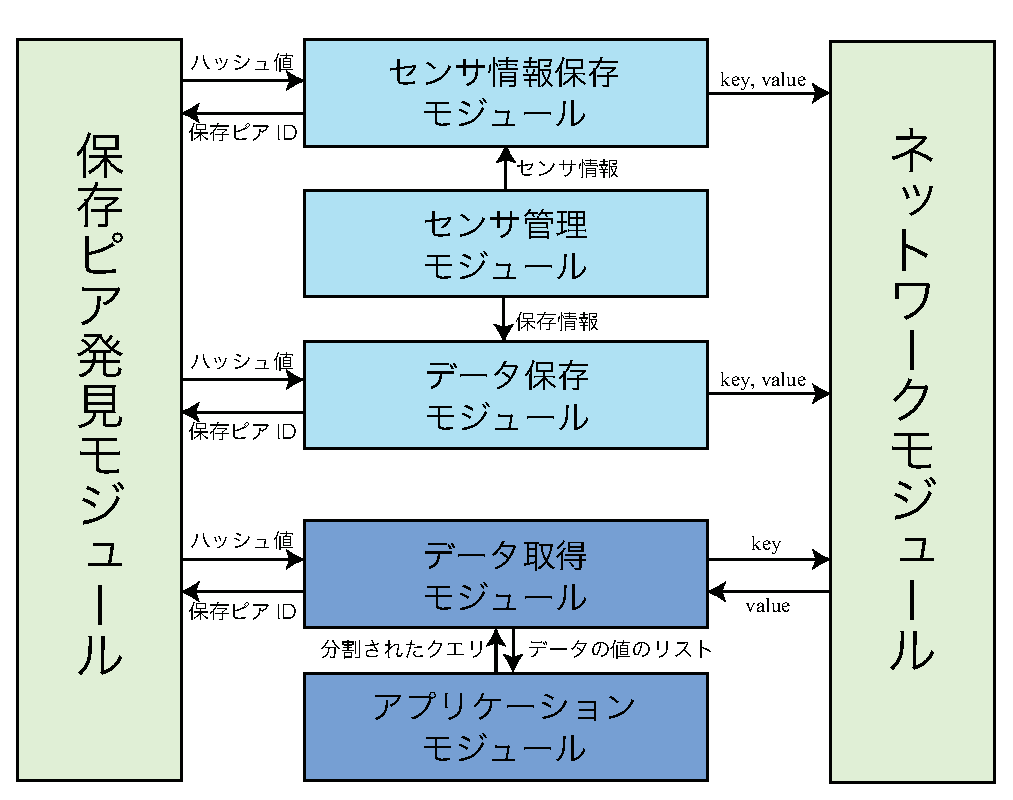
\includegraphics[width=130mm]{./images/sysconf.eps}
 \end{center}
 \caption{システム構成図}
 \label{fig:sysconf}
\end{figure}

\subsection{ネットワークモジュール}
ネットワークモジュールは保存ピア同士で協調し,1Dトーラス型のオーバーレイネットワークを構築及びデータに関する通信を行うモジュールである.本モジュールでは,他の保存ピアのデータ取得モジュールから,データ取得のクエリが送られた場合に,対象のデータをクエリ送信元の保存ピアに送信する.

本モジュールの実装はオープンソースであるOpenChordの一部を参考にしている.保存ピアのJoin,Retrieveなどの保存ピアによるネットワークの構築の部分において利用している.

\subsection{センサ情報管理モジュール}
本モジュールは,センサの緯度や経度など,センサデータの値以外の多次元データとしてのセンサ情報を適切な場所に保存することで,データの取得を可能にするモジュールである.

センサデータの取得を考えた際に,一般的な手法は,センサノードのアドレスを指定して取得するが,T-Ringが想定している環境では,センサデータをアドレス以外の他の要素から取得する.よって,取得を行う時には,取得されるセンサデータの情報が必要である.このために,T-Ringでは,対象のセンサノードの緯度,経度,センサタイプ,マスターピア=0で一次元化,ハッシュ化した値を担当する保存ピアに対して,このセンサ情報を登録する.登録はセンサデータの値の保存と同様に行う.センサデータの保存については,次節で詳細に述べる.保存におけるキーとして,緯度,経度,センサタイプ,マスターピア=0の4次元値を1次元化,ハッシュ化した値を,バリューとして,そのセンサのchunkとSPの時間のセットを保存する.データの取得については,5.4で詳細に述べるが,データの取得の際には,緯度,経度,センサタイプ,chunk,SPの時間を必要とする.緯度,経度,センサタイプ,マスターピア=0の担当ピアに取得に必要なセンサ情報を登録することによって,chunkとSPの時間を知ることが可能になる.

本モジュールでは,最初に,センサに関する情報が登録されているSensorInfo.csvから,センサIDをキーとして,センサデータの保存に必要である,緯度,経度,センサタイプ,chunk,SPの時間を取得する.取得された情報から,緯度,経度,センサタイプ,マスターピア=0の4次元値をZ-order関数によって処理し,返されたバイナリ値を保存ピア発見モジュールに渡す.保存ピア発見モジュールは,担当の保存ピアの保存ピアIDを返してくるので,そのピアに対して必要な情報を登録する.
\if0
\begin{lstlisting}[caption=センサ情報の登録]

public class StoreSensorInformationThread extends Thread {
	private String sensorId;
	private String fileName;
	private String tmpName;
	private FileProcessor fileProcessor;
	private File tmp;
	private InformationDeliveryInterface informationDelivery;

	public StoreSensorInformationThread(JoinData joinData, String id) {
		this.sensorId = id;
		this.fileName = "sensorInfo.csv";
		this.tmpName = "sensorInfo.tmp";
		this.fileProcessor = new FileProcessor(fileName, tmpName);
		this.tmp = new File(tmpName);
		this.informationDelivery = new InformationDeliveryImpl(joinData);
	}
	
	public void run(){
		SensorInformation sensorInformation = new SensorInformation();
		
		long getLineNum = 0;
		getLineNum = fileProcessor.searchLine(sensorId, tmp);
		
		String[] sensorInfoList = null;
		
		sensorInfoList = fileProcessor.getLine(getLineNum);
		
		if (sensorInfoList != null) {
			for (int i = 0; i < sensorInfoList.length; i++) {
				switch(i){
				case 1:
					long latitude = Long.parseLong(sensorInfoList[i]);
					sensorInformation.latitude = latitude;
					break;
				case 2:
					long longitude = Long.parseLong(sensorInfoList[i]);
					sensorInformation.longitude = longitude;
					break;
				case 3:
					long sensorType = Long.parseLong(sensorInfoList[i]);
					sensorInformation.type = sensorType;
					break;
				case 4:
					long chunkTime = Long.parseLong(sensorInfoList[i]);
					sensorInformation.chunk = chunkTime;
					break;
				case 5:
					long startPointTime = Long.parseLong(sensorInfoList[i]);
					sensorInformation.startPoint = startPointTime;
					break;
				case 7:
					long configTime = Long.parseLong(sensorInfoList[i]);
					sensorInformation.configTime = configTime;
					break;
				}
			}
		} else {
			System.out.println(sensorId + " isn't in " + fileName);
		}
		informationDelivery.storeSensorInformation(sensorInformation);
	}
}
\end{lstlisting}
\fi
\subsection{データ保存モジュール}
本モジュールはセンサデータを保存する保存するモジュールである.

T-Ringでは,センサデータの時間に従って保存先を決めるため,センサ管理モジュールから,センサID,対象データの緯度,経度,センサタイプ,chunk,SPの時間,データの時間,センサの設定時間を取得する.本モジュールでは,フィールドとして,センサIDをキーに,次に保存すべき保存ピアのIDをバリューとするMapを所持している.送られてきたセンサIDとMap内のセンサIDを比較し,登録されていない場合は,データの時間,センサの設定時間,chunkから,まず,マスターピアの番号を決定する.次いで,そのマスターピアからSuccessorを辿る回数を計算する.そして,緯度,経度,センサタイプ,マスターピアの番号の4次元からハッシュ化をし,その値とSuccessorを辿る回数を保存ピア発見モジュールに送る.その結果として保存ピアIDを受け取る.データが保存されるセンサのIDとMap内のセンサIDが一致していた場合は,そのMapのセンサIDに対応する保存ピアのIDを取得する.次に,そのIDの保存ピアに対して,キーを緯度,経度,センサタイプの1次元化とハッシュ値,バリューをデータの値として保存する.

また,保存が行われると,次に保存するべき保存ピアの計算が行われる.ここからはセンサのIDとデータの時間だけを監視する.この計算を行うために,センサIDをキーとして,最新のセンサデータが保存された保存ピアのID,マスターピアの番号それぞれをバリューとして保存する2つのフィールドが存在する.次に送られてきたデータが前回のデータと比較してchunkが異なっていた場合,保存ピア発見モジュールに対して,最新の保存データが保存された保存ピアIDとSuccessorを辿る回数が送られる.これに対して,対象の保存ピアのIDが返される.この保存ピアのIDを次に保存すべき保存ピアIDとして更新する.次に,chunkが同一であった場合,最新の保存データが保存された保存ピアIDを次に保存すべき保存ピアIDをとして更新する.マスターピアが異なっていた場合,センサIDが登録されていない時と同様の処理を行い,保存ピア発見モジュールから返された保存ピアIDを次に保存すべき保存ピアIDとして更新する.

これらの処理が繰り返えされることにより,データの保存が行われる.以上に述べた処理をフローチャートで示す.

\subsection{データ取得モジュール}
アプリケーションモジュールから送られるユーザからの取得のクエリは,範囲を持ったクエリであるので,本モジュールにより,クエリの緯度,経度,半径から分割を行う.これについては図\ref{fig:divide}が例と図解である.そして,分割を行ったそれぞれの位置について,緯度,経度,センサタイプとクエリで指定された取得時間から,データ保存と同じ手順により,緯度,経度,センサタイプ,マスターピアの番号の4次元によるハッシュ値,Successorを辿る回数を保存ピア発見モジュールに送り,その結果として受け取った保存ピアIDに対して,緯度,経度,センサタイプで生成されるキーからバリューを受け取る.この受け取ったバリューのセットを,指定された方式に変換しアプリケーションモジュールに送り返す.指定された方式に関しては,アプリケーションモジュールの解説の際に説明する.

\begin{figure}[htbp]
 \begin{center}
  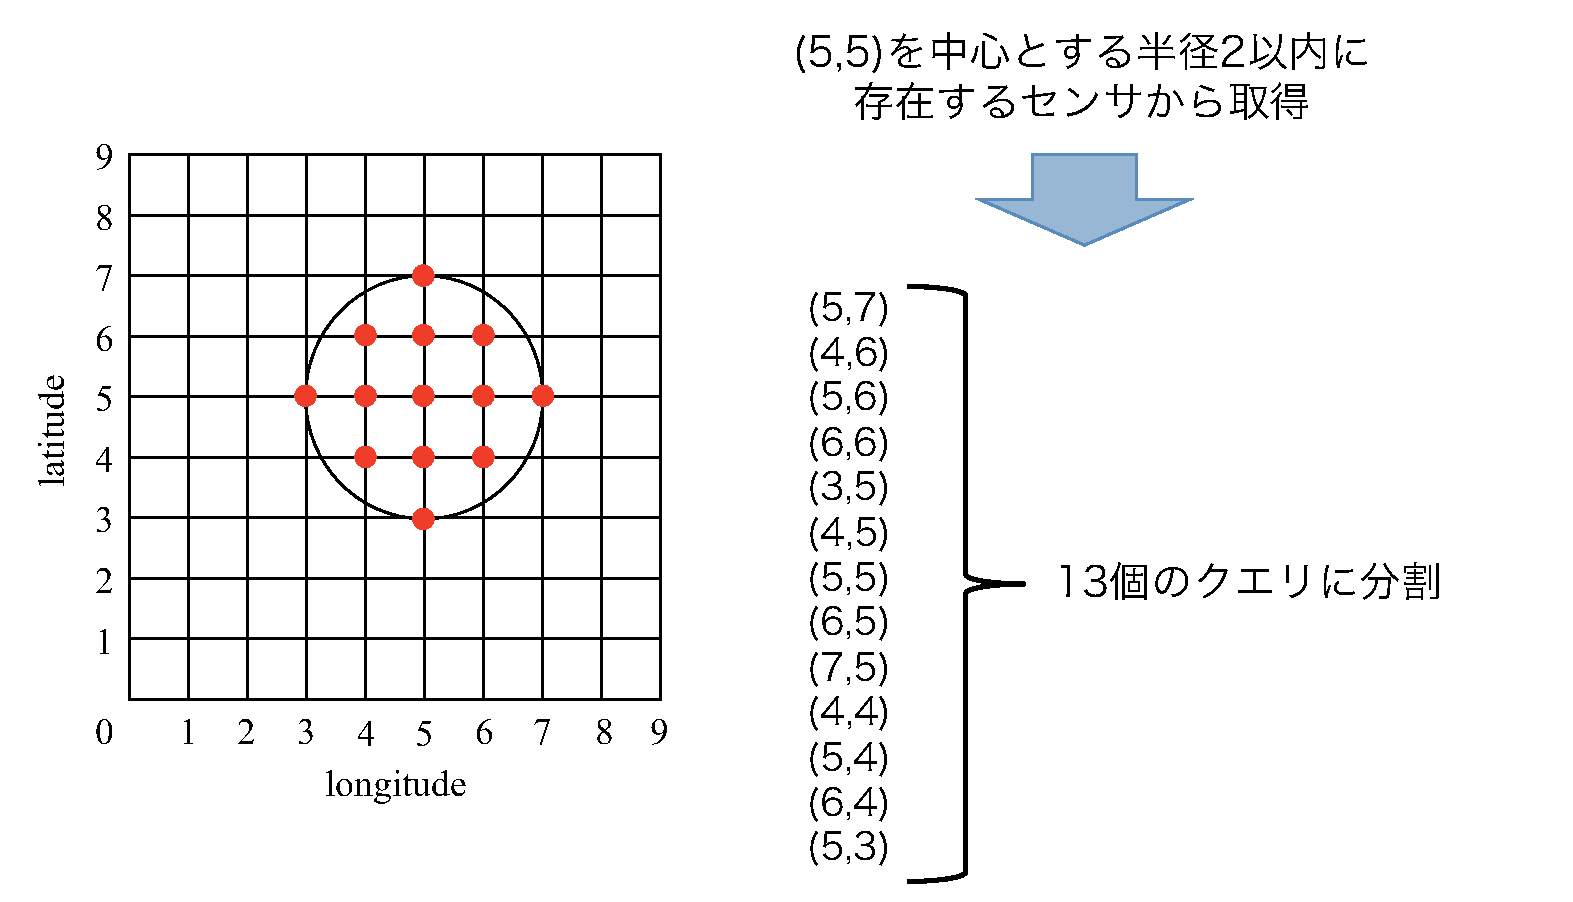
\includegraphics[width=130mm]{./images/divide.eps}
 \end{center}
 \caption{クエリの分割}
 \label{fig:divide}
\end{figure}

\subsection{保存ピア発見モジュール}
本モジュールは,センサ情報管理モジュール,データ保存モジュール,データ取得モジュールから受け取ったハッシュ値やSuccessorを辿る回数から,対象の保存ピアを発見し,そのアドレスを各モジュールに送り返す.

T-Ringでは2種類の保存ピアの発見の方法が存在する,1つ目は,Finger Tableを用いた発見である.Finger Tableの計算回数は$O(\log{2}N)$である.この発見はデータ保存モジュール,データ取得モジュールから送られた緯度,経度,センサタイプ,マスターピアの番号の4次元によるハッシュ値が前データと異なる場合に,マスターピアを探索するために行われる.また,Synapseにおける保存,取得では,センサデータ毎にこの計算がなされる.

2つ目の方法は,データ保存モジュール,データ取得モジュールから送られた緯度,経度,センサタイプ,マスターピアの番号の4次元によるハッシュ値が前データと同様であった場合に行われる.この場合,前データで取得したアドレスのSuccessorのアドレスを取得する.Finger Tableによる計算は前データの際に行ったため,計算回数は$O(1)$である.

これらの方法により発見されたアドレスをデータ保存モジュール,データ取得モジュールに送り返す.

\begin{lstlisting}[caption=データ保存時の保存ピア発見]
public class NextStorePeer {
	private TRingImpl tring;
	private HashMap<String, Node> nextNode;
	private HashMap<String, Long> restTime;
	private HashMap<String, Long> prevSP;
	private HashMap<String, Long> prevTime;
	ArrayList<Long> positions;

	public NextStorePeer(JoinData joinData) {
		this.positions = new ArrayList<Long>();
		this.nextNode = new HashMap<String, Node>();
		this.restTime = new HashMap<String, Long>();
		this.prevSP = new HashMap<String, Long>();
		this.prevTime = new HashMap<String, Long>();
		this.tring = joinData.tring;
	}

	public synchronized Node getNextStorePeer(Node node, DataForStore data,
			Key key) throws CommunicationException {
		setNextStorePeer(node, data, key);
		return nextNode.get(Arrays.toString(key.getBytes()));
	}

	private synchronized void setNextStorePeer(Node currentPeer,
			DataForStore data, Key key) throws CommunicationException {
		long SP = (data.time - data.configTime) / data.startPoint;

		if (nextNode.get(Arrays.toString(key.getBytes())) == null) {
			this.nextNode
					.put(Arrays.toString(key.getBytes()), currentPeer
							.findSuccessor(currentPeer.getNodeAddingOneID()));
			this.prevSP.put(Arrays.toString(key.getBytes()), SP);
			this.restTime.put(Arrays.toString(key.getBytes()), data.startPoint
					- data.chunk);
		} else {
			if (this.prevSP.get(Arrays.toString(key.getBytes())) != SP) {
				this.positions.add(data.latitude);
				positions.add(data.longitude);
				positions.add(data.type);
				this.positions.add(SP);
				ZorderInterface zorder = new Zorder(positions);
				byte[] SPKey = zorder.getZorder();
				Key masterPeerKey = new ByteArrayKey(SPKey);
				nextNode.put(Arrays.toString(key.getBytes()),
						tring.getResponsiblePeer(masterPeerKey));
				this.prevSP.put(Arrays.toString(key.getBytes()), SP);
			} else if (restTime.get(Arrays.toString(key.getBytes()))
					- data.chunk > 0) {
				this.nextNode.put(Arrays.toString(key.getBytes()), currentPeer
						.findSuccessor(currentPeer.getNodeAddingOneID()));
			}
			this.restTime.put(Arrays.toString(key.getBytes()), data.startPoint
					- data.chunk);
		}
	}
}
\end{lstlisting}

\begin{lstlisting}[caption=データ取得時の保存ピア発見]

public class NextRetrievePeer {
	private TRingImpl tring;
	private HashMap<String, Node> nextNode;
	private HashMap<String, Long> restTime;
	private HashMap<String, Long> prevSP;
	ArrayList<Long> retrievedData;
	ArrayList<Long> positions;

	public NextRetrievePeer(TRingImpl tring) {
		this.positions = new ArrayList<Long>();
		this.nextNode = new HashMap<String, Node>();
		this.restTime = new HashMap<String, Long>();
		this.prevSP = new HashMap<String, Long>();
		this.retrievedData = new ArrayList<Long>();
		this.tring = tring;
	}

	public synchronized ArrayList<Long> getNextRetrievePeer(
		DataForRetrieve data, long latitude, long longitude,
		HashMap<String, Long> sensorInfo, Key key)
		setNextRetrievePeer(data, latitude, longitude, sensorInfo, key);
		return this.retrievedData;
	}

	private synchronized void setNextRetrievePeer(DataForRetrieve data,
			long latitude, long longitude, HashMap<String, Long> sensorInfo,
			Key key) throws CommunicationException {
		String tag = Arrays.toString(key.getBytes());
		long currentTime = data.timeFrom;
		long SPTime = sensorInfo.get("SP");
		long chunk = sensorInfo.get("chunk");
		long configTime = sensorInfo.get("configTime");
		long SP = (currentTime - configTime) / SPTime;
		long pastTime = currentTime - configTime - (SP * SPTime);
		long leftChangeTime = SPTime - pastTime;
		long leftTime = data.timeTo - currentTime;

		ArrayList<Long> positions = new ArrayList<Long>();
		positions.add(latitude);
		positions.add(longitude);
		positions.add(data.type);
		positions.add(SP);
		ZorderInterface zorder = new Zorder(positions);
		byte[] SPKey = zorder.getZorder();
		Key masterPeerKey = new ByteArrayKey(SPKey);

		nextNode.put(tag, tring.getResponsiblePeer(masterPeerKey));

		Node currentNode = nextNode.get(tag);

		while (leftTime > 0) {
			leftTime -= chunk;
			leftChangeTime -= chunk;

			if (leftChangeTime > 0) {
				this.retrievedData.addAll(tring.retrieveData(key,
						this.nextNode.get(tag)));
				this.nextNode.put(
						tag,
						this.nextNode.get(tag).findSuccessor(
				this.nextNode.get(tag).getNodeAddingOneID()));
				
			} else {
				leftChangeTime += SPTime;
				positions.set(3, positions.get(3) + 1);
				zorder = new Zorder(positions);
				SPKey = zorder.getZorder();
				masterPeerKey = newByteArrayKey(SPKey);
				this.nextNode.put(tag,this.nextNode.get(tag).findSuccessor(this.nextNode.get(tag).getNodeAddingOneID()));	
				this.retrievedData.addAll(tring.retrieveData(key,this.nextNode.get(tag)));
				
			}
		}
	}
}
\end{lstlisting}

\subsection{センサ管理モジュール}
本モジュールはセンサネットワーク内のセンサ毎の緯度,経度,センサタイプ,などを管理を行うモジュールである.センサが環境に設置された際に,そのセンサの情報を所属する保存ピアへ登録する.また,センサの移動により,緯度,経度の変更が発生した際に,その情報を更新する.

センサが環境に設置を行う際,以下のようなセンサ情報登録クラスのインスタンスを用いてSensorInfo.csvに登録を行う.SensorInfo.csvに登録されるエントリは,各センサごとに,sensorId,latitude,longitude,sensorType,chunkTime,startPointTimeである.センサの設置場所が変更された際は,sensorIdから対象のエントリを発見し,変更を行う.このSensorInfo.csvの情報は,センサ情報保存モジュール,データ保存モジュールで利用される.以下がセンサ情報の登録,変更のメインクラスである.
\if0
\begin{lstlisting}[caption=センサ情報の保存,変更]

public class SensorInfo {
	private String fileName;
	private String tmpName;
	private FileProcessor fileProcessor;
	private int num;
	
	public SensorInfo(String fileName, String tmpName) {
		this.fileName = fileName;
		this.tmpName = tmpName;
		this.fileProcessor = new FileProcessor(fileName, tmpName);
		this.num = 0;
	}

	public void add(String sensorId, long latitude, long longitude, long sensorType, long chunkTime, long startPointTime){
			fileProcessor.insert(sensorId, latitude, longitude, sensorType, chunkTime, startPointTime);
		}
	}
	
	public void changeLatitude(String sensorId, long latitude) {
		num = 1;
		String prevValue = fileProcessor.changeElement(sensorId, latitude, num);
	}

	public void changeLongitude(String sensorId, long longitude) {
		num = 2;
		String prevValue = fileProcessor.changeElement(sensorId, longitude, num);
	}

	public void changeSensorType(String sensorId, long sensorType) {
		num = 3;
		String prevValue = fileProcessor.changeElement(sensorId, sensorType, num);
	}
	
	public void changeChunkTime(String sensorId, long chunkTime){
		num = 4;
		String prevValue = fileProcessor.changeElement(sensorId, chunkTime, num);
	}
	
	public void changeStartPointTime(String sensorId, long startPointTime){
		num = 5;
		String prevValue = fileProcessor.changeElement(sensorId, startPointTime, num);
	}	

	public void remove(String sensorId){
		fileProcessor.delete(sensorId);
	}
}
 
\end{lstlisting}
\fi

\subsection{アプリケーションモジュール}
本モジュールはユーザアプリケーションに対してのデータ取得のインターフェースを提供し,ユーザアプリケーションは5.1.1で述べたクエリを本モジュールに送信する.本モジュールとはTCPで通信を行い.7777番ポートを利用する.ユーザアプリケーションとのセッションが確立し,クエリの受信が完了すると,データ取得モジュールにこのクエリをフォワードし,その結果をユーザアプリケーションが指定した方式で送り返す.この方式の指定には4つの方法があり,指定領域内の全データのリスト,最大値,最小値,平均値である.


\section{まとめ}
本章では,まず,ソフトウェアの構成について述べた,そして,個々のモジュールの細かな設計と実装について述べた.特に重要なアルゴリズムについては,各小節の末尾に実際のプログラムを掲載した.
\chapter{評価}
\begin{large}
\begin{quote}
本章では,T-Ringシステムの評価を行う.
\end{quote}
\end{large}
\clearpage

\section{評価方針}
本研究では,センサデータを多次元データとして扱う際に,時間を他の属性と同様に扱っているSynapseと,センサデータの時間的特殊性を考慮したT-Ringの取得時間の比較を行う.
Synapseの手法では,保存,取得の際に,データごとにFinger Tableによる保存ピアの探索を行わなければならない.よって,本評価では,ネットワークに参加するピア数を固定し,データの保存,取得に共通する,保存ピア探索の計算コストを計測する.次に,保存時,取得時に分けて探索に要する時間の計測を行う.
%本研究に評価では,まず,ネットワークに参加する保存ピアの数を固定し,単位時間における取得のクエリ数を段階的に増やし,全ての情報の取得が終了するまでにどれだけの時間がかかるかを評価する.次に,ネットワーク内の保存ピア数により,一回の保存ピア探索のホップ数が変化するので,単位時間における取得のクエリ数を固定し,ネットワークに参加する保存ピアの数を変化させる.
%取得の対象データは,評価結果に影響を与えないが,センサデータであることを考慮し,サイズは2バイトとする.

\section{評価環境}
本研究は,評価環境として,慶応義塾大学湘南藤沢キャンパス内の特別教室内に設置されている124台のiMacの内,任意の複数マシンを用いて行う.詳細なスペックなどについては以下の表\ref{tab:information}で示す.

\begin{table}[htb]
  \centering
  \caption{実験環境}
  \begin{tabular}{|c||c|} \hline
  	ホスト名	 & zmac000-159 \\ \hline
	本体 & iMac 21.5 インチ \\ \hline
	CPU	& 3.06 GHz Intel Core 2 Duo \\ \hline
	メモリ & 4 GB (2 GB X 2) \\ \hline
	ハードディスク	& 499.76 GB \\ \hline
	OS & Mac OS X 10.6.5 \\ \hline
  \end{tabular}
  \label{tab:information}
\end{table}
\subsection{実験環境内におけるネットワークレイテンシ}
本研究では,データの保存や探索に要する時間を計測するため,各保存ピア間の通信におけるレイテンシが重要になる.そこで,本実験環境におけるマシン間のレイテンシが実験にどの程度の影響を与えるのかを調査するため,事前実験として,各リージョン間のRTTを計測した.各リージョンがどこに存在するかは,図\ref{fig:region}において示す.それぞれICMPにおけるEcho Messageを送信し,リプライが返されるまでの時間の計測を100回行い,その平均値,最小値,最大値,標準偏差を表\ref{tab:ping_regionA},\ref{tab:ping_regionB},\ref{tab:ping_regionC},\ref{tab:ping_regionD}で示す.本実験において,実験環境下ではRTTが0.400ms以下であるという知見が得られた.本システムが用いられる実環境におけるRTTは0.400msより十分に大きいため,本評価では,実験環境内におけるネットワークレイテンシを無視する.


 \begin{figure}[htbp]
 %\begin{minipage}{0.5\hsize}
  \begin{center}
   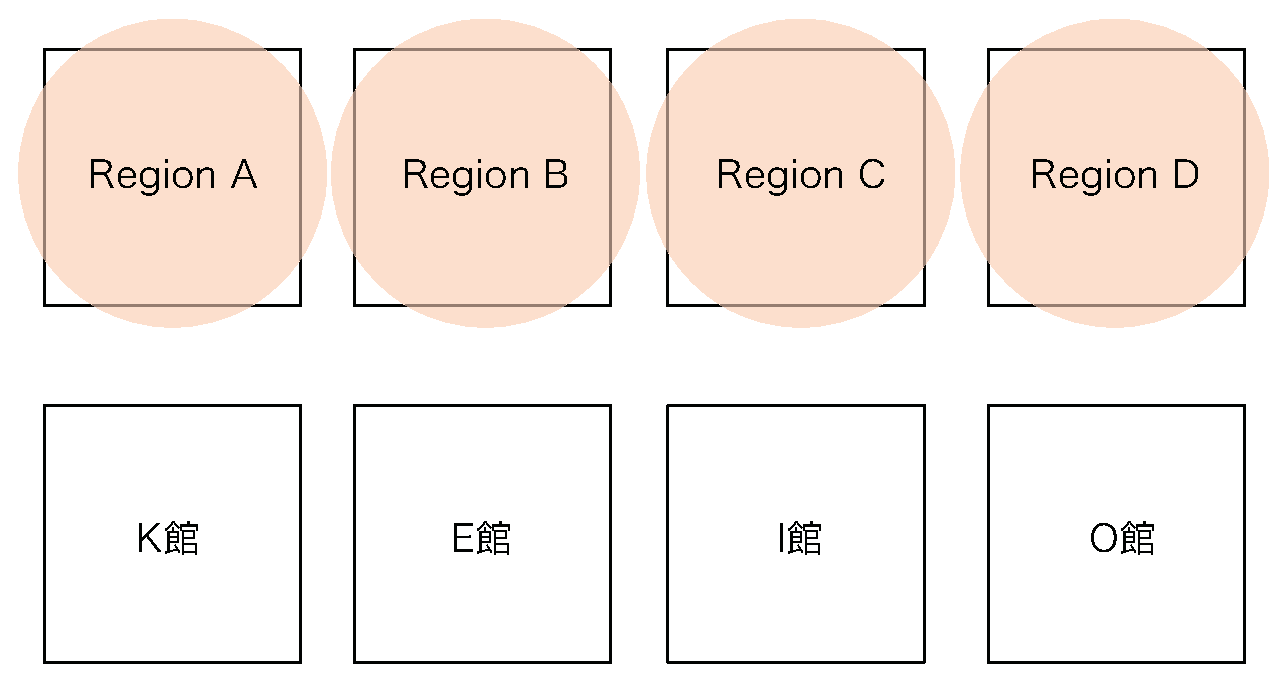
\includegraphics[width=140mm]{./images/region.eps}
  \end{center}
  \caption{リージョンの関係性}
  \label{fig:region}
 %\end{minipage}
\end{figure}

%\begin{table}[htb]
%  \centering
%  \caption{リージョンAからのRTT}
%  \begin{tabular}{|c||c|c|c|c|} \hline
%    \backslashbox{}{} & 平均値 & 最小値 & 最大値 & 標準偏差 \\ \hline \hline
%    リージョンA & 0.234 ms & 0.193 ms & 0.271 ms & 0.022 \\ \hline
%    リージョンB & 0.324 ms & 0.287 ms & 0.349 ms & 0.015 \\ \hline
%    リージョンC & 0.321 ms & 0.285 ms & 0.347 ms & 0.016 \\ \hline
%    リージョンD & 0.315 ms & 0.277 ms & 0.339 ms & 0.016 \\ \hline
%  \end{tabular}
%  \label{tab:ping_regionA}
%\end{table}

%\begin{table}[htb]
%  \centering
%  \caption{リージョンBからのRTT}
%  \begin{tabular}{|c||c|c|c|c|} \hline
%    \backslashbox{}{} & 平均値 & 最小値 & 最大値 & 標準偏差 \\ \hline \hline
%    リージョンA & 0.327 ms & 0.288 ms & 0.347 ms & 0.015 \\ \hline
%    リージョンB & 0.238 ms & 0.203 ms & 0.270 ms & 0.019 \\ \hline
%    リージョンC & 0.319 ms & 0.274 ms & 0.349 ms & 0.018 \\ \hline
%    リージョンD & 0.317 ms & 0.282 ms & 0.347 ms & 0.015 \\ \hline
%  \end{tabular}
%  \label{tab:ping_regionB}
%\end{table}

%\begin{table}[htb]
%  \centering
%  \caption{リージョンCからのRTT}
%  \begin{tabular}{|c||c|c|c|c|} \hline
%    \backslashbox{}{} & 平均値 & 最小値 & 最大値 & 標準偏差 \\ \hline \hline
%    リージョンA & 0.325 ms & 0.277 ms & 0.359 ms & 0.016 \\ \hline
%    リージョンB & 0.312 ms & 0.279 ms & 0.342 ms & 0.015 \\ \hline
%    リージョンC & 0.252 ms & 0.192 ms & 0.379 ms & 0.022 \\ \hline
%    リージョンD & 0.319 ms & 0.283 ms & 0.343 ms & 0.015 \\ \hline
%  \end{tabular}
%  \label{tab:ping_regionC}
%\end{table}

%\begin{table}[htb]
%  \centering
%  \caption{リージョンDからのRTT}
%  \begin{tabular}{|c||c|c|c|c|} \hline
%    \backslashbox{}{} & 平均値 & 最小値 & 最大値 & 標準偏差 \\ \hline \hline
%    リージョンA & 0.296 ms & 0.240 ms & 0.727 ms & 0.047 \\ \hline
%    リージョンB & 0.295 ms & 0.259 ms & 0.374 ms & 0.014 \\ \hline
%    リージョンC & 0.252 ms & 0.192 ms & 0.379 ms & 0.022 \\ \hline
%    リージョンD & 0.291 ms & 0.239 ms & 0.335 ms & 0.013 \\ \hline
%  \end{tabular}
%  \label{tab:ping_regionD}
%\end{table}

\section{保存ピア探索の計算コスト}
データの保存,取得時に,Synapseでは対象のデータの時間毎に保存ピアの探索を行う一方で,T-Ringは対象のセンサーのchunk,SPの値により,探索の回数が変化する.そこで,1000個の連続したデータを保存,取得することを想定し,Synapse,T-Ringの両手法において,1データの平均のピア間ホップ数を計測する.またT-Ringにおいては,各データの時間の間隔を5,SPを100,chunkを10,30,50,70,90の5つとする.図\ref{fig:compare_hop}はその結果である.

 \begin{figure}[htbp]
 %\begin{minipage}{0.5\hsize}
  \begin{center}
   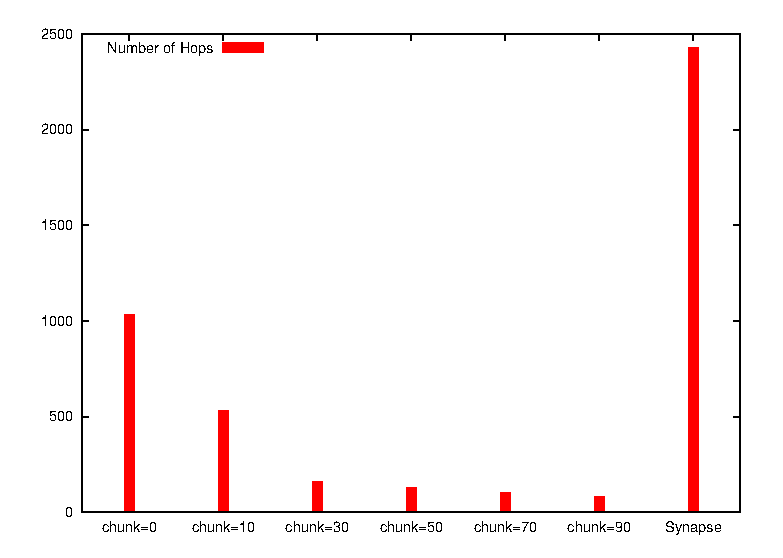
\includegraphics[width=130mm]{./images/compare_hop.eps}
  \end{center}
  \caption{ホップ数}
  \label{fig:compare_hop}
 %\end{minipage}
\end{figure}



\section{データ保存時の評価}
データの保存時にSynapseでは,データ毎に保存場所の計算を行う.その一方で,T-Ringでは,ある一定の時間が経過するまでは,保存場所の変更が発生しない.そこで,ある保存ピアに100個のデータを保存するクエリを送り,それらの保存が完了するまでの時間を計測する.本評価では,保存されるデータの設定をchunk=30,SP=100,各データの時間の間隔を5として実験を行った.また,ネットワークの環境については,ネットワークに参加している保存ピアの数(ネットワークサイズ=NS)を10,50,100の3種類,各ピア間のRTTを5,10,50,1000の4種類とした.図\ref{fig:compare_store_rtt5},\ref{fig:compare_store_rtt10},\ref{fig:compare_store_rtt50},\ref{fig:compare_store_rtt100}はRTTごとにまとめた実験結果である.

%\begin{figure}[htbp]
%\begin{minipage}{1\textwidth}
%    \centering
%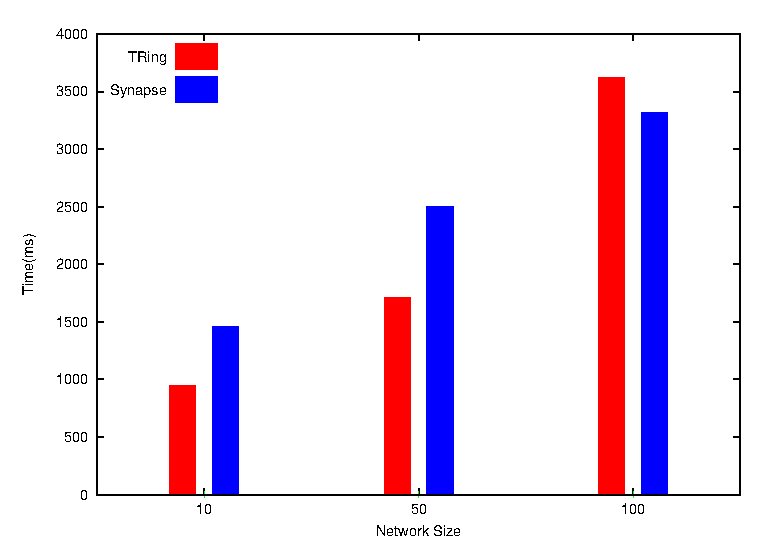
\includegraphics[width=14cm]{./images/compare_store_rtt5.eps}
%\begin{center}
%  \begin{tabular}{|c||c|c|c|} \hline
%    \backslashbox{}{} & NS=10 & NS=50 & NS=100  \\ \hline \hline
%       T-Ring & 944 ms & 1708 ms & 3625 ms  \\ \hline
%       Synapse & 1458  ms & 2506 ms & 3315 ms \\ \hline
%  \end{tabular}
%\end{center}
%\caption{保存:RTT=5}
% \label{fig:compare_store_rtt5}
% \end{minipage}
%\end{figure}


%\begin{figure}[htbp]
%\begin{minipage}{1\textwidth}
%    \centering
%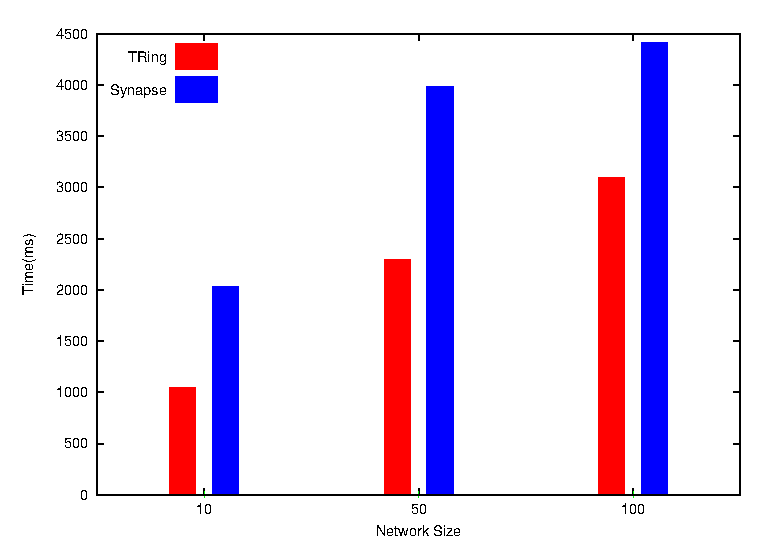
\includegraphics[width=14cm]{./images/compare_store_rtt10.eps}
% \begin{center}
% %\begin{table}[htbp]
%  %\centering
%  %\caption{保存:RTT=10値}
%  \begin{tabular}{|c||c|c|c|} \hline
%    \backslashbox{}{} & NS=10 & NS=50 & NS=100  \\ \hline \hline
%       T-Ring & 1049 ms & 2300 ms & 3101 ms  \\ \hline
%       Synapse & 2029  ms & 3989 ms & 4414 ms \\ \hline  \end{tabular}
%  \label{tab:RTT=10}
%\end{center}
%\caption{保存:RTT=10}
% \label{fig:compare_store_rtt10}
% \end{minipage}
%\end{figure}

%\begin{figure}[htbp]
%\begin{minipage}{1\textwidth}
%    \centering
%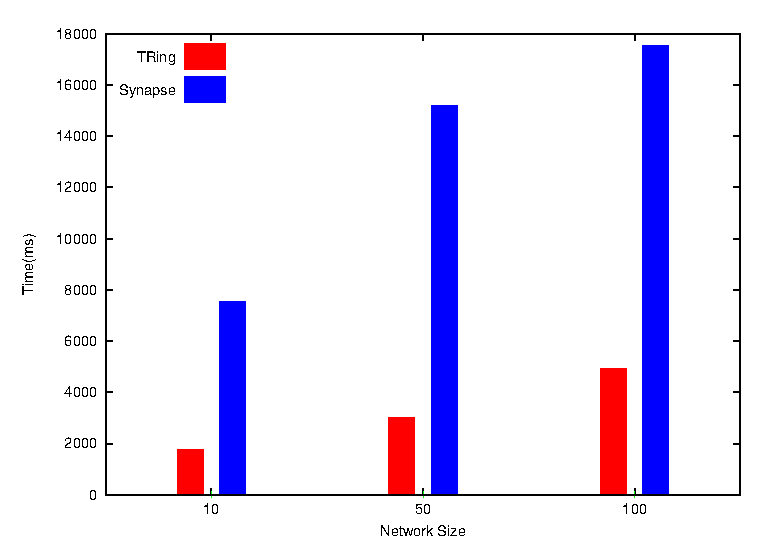
\includegraphics[width=14cm]{./images/compare_store_rtt50.eps}
%\begin{center}
% %\begin{table}[htbp]
%  %\centering
%  %\caption{保存:RTT=50値}
%  \begin{tabular}{|c||c|c|c|} \hline
%    \backslashbox{}{} & NS=10 & NS=50 & NS=100  \\ \hline \hline
%       T-Ring & 1049 ms & 2300 ms & 3101 ms  \\ \hline
%       Synapse & 2029  ms & 3989 ms & 4414 ms \\ \hline  \end{tabular}
%  \label{tab:RTT=50}
%\end{center}
%\caption{保存:RTT=50}
%\label{fig:compare_store_rtt50}
% \end{minipage}
%\end{figure}

%\begin{figure}[htbp]
%\begin{minipage}{1\textwidth}
%    \centering
%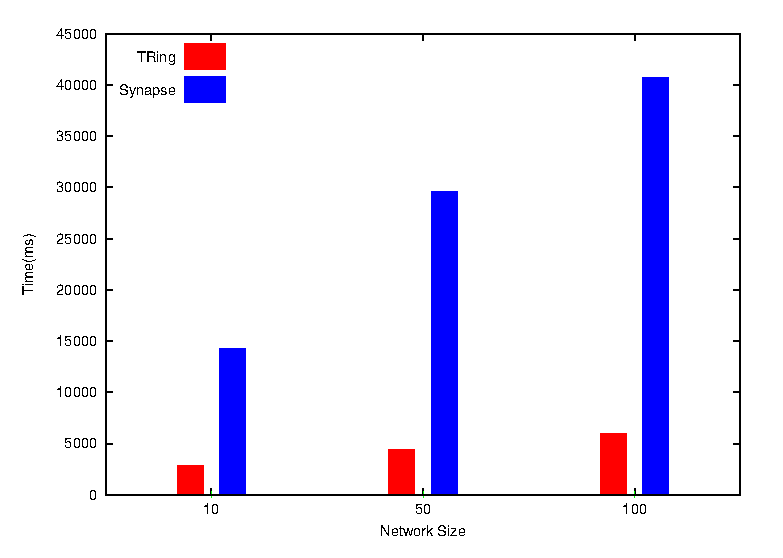
\includegraphics[width=14cm]{./images/compare_store_rtt100.eps}
%%\caption{保存:RTT=100}
%\begin{center}
% %\begin{table}[htbp]
%  %\centering
%  %\caption{保存:RTT=100値}
%  \begin{tabular}{|c||c|c|c|} \hline
%    \backslashbox{}{} & NS=10 & NS=50 & NS=100  \\ \hline \hline
%       T-Ring & 1049 ms & 2300 ms & 3101 ms  \\ \hline
%       Synapse & 2029  ms & 3989 ms & 4414 ms \\ \hline  \end{tabular}
%  \label{tab:RTT=100}
%\end{center}
%\caption{保存:RTT=100}
%\label{fig:compare_store_rtt100}
% \end{minipage}
%\end{figure}




\section{データ取得時の評価}
保存時と同様に,データの取得時にSynapseでは,取得するセンサデータごとに保存場所の探索を行い,T-Ringではある一定の時間が経過するまで,取得先の変更は発生しない.そこで,ある特定の領域に対して,500単位時間のデータの取得を行うクエリを送り,データが全て返されるまでの時間を計測する.本評価では,データはすべて5単位時間ごとに保存されている環境を想定する.よって,500単位時間分のデータは,100個のデータを取得することとなる.クエリの地理的範囲は半径10の広さを持ったものとする.また,ネットワークに関しては,保存時と同様に,ネットワークに参加している保存ピアの数(ネットワークサイズ=NS)を10,50,100の3種類,各ピア間のRTTを5,10,50,1000の4種類とした.図\ref{fig:compare_retrieve_rtt5},\ref{fig:compare_retrieve_rtt10},\ref{fig:compare_retrieve_rtt50},\ref{fig:compare_retrieve_rtt100}はRTTごとにまとめた実験結果である.
%保存場所探索の計算が行われた回数,データが保存されているピアを発見に至るホップ数の総計,取得の開始から完了までの時間を計測する.また,単位時間を1分とし,クエリの送信回数を100回から10000回に漸次的に増加させる.

%\begin{figure}[htbp]
%\begin{minipage}{1\textwidth}
%    \centering
%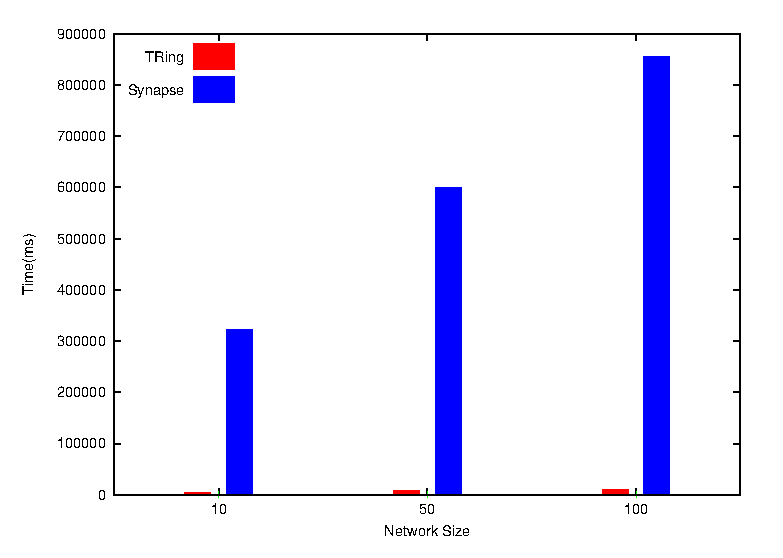
\includegraphics[width=14cm]{./images/compare_retrieve_rtt5.eps}
%\begin{center}
%  \begin{tabular}{|c||c|c|c|} \hline
%    \backslashbox{}{} & NS=10 & NS=50 & NS=100  \\ \hline \hline
%       T-Ring & 3884 ms & 8098 ms & 9823 ms  \\ \hline
%       Synapse & 322615  ms & 599557 ms & 855187 ms \\ \hline
%  \end{tabular}
%\end{center}
%\caption{取得:RTT=5}
% \label{fig:compare_retrieve_rtt5}
% \end{minipage}
%\end{figure}

%\begin{figure}[htbp]
%\begin{minipage}{1\textwidth}
%    \centering
%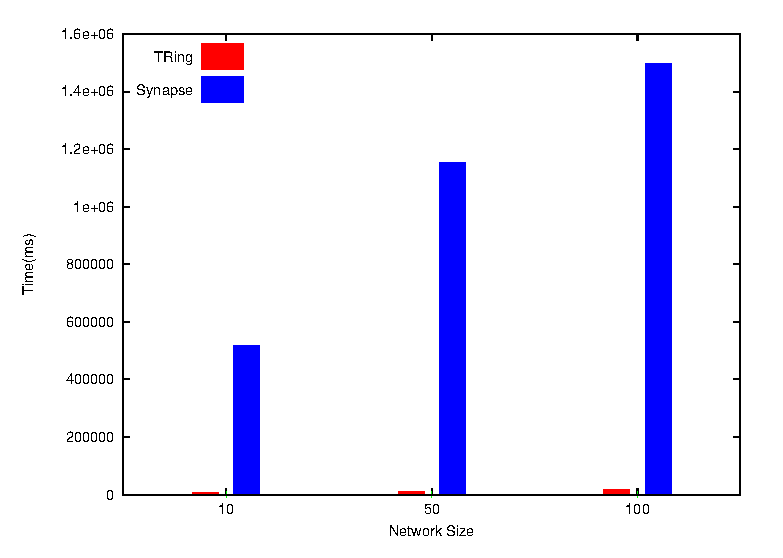
\includegraphics[width=14cm]{./images/compare_retrieve_rtt10.eps}
%\begin{center}
%  \begin{tabular}{|c||c|c|c|} \hline
%  \backslashbox{}{} & NS=10 & NS=50 & NS=100  \\ \hline \hline
%       T-Ring & 6247 ms & 12683 ms & 16249 ms  \\ \hline
%       Synapse & 519541  ms & 1155219 ms & 1498550 ms \\ \hline
%  \end{tabular}
%\end{center}
%\caption{取得:RTT=10}
% \label{fig:compare_retrieve_rtt10}
% \end{minipage}
%\end{figure}

%\begin{figure}[htbp]
%\begin{minipage}{1\textwidth}
%    \centering
%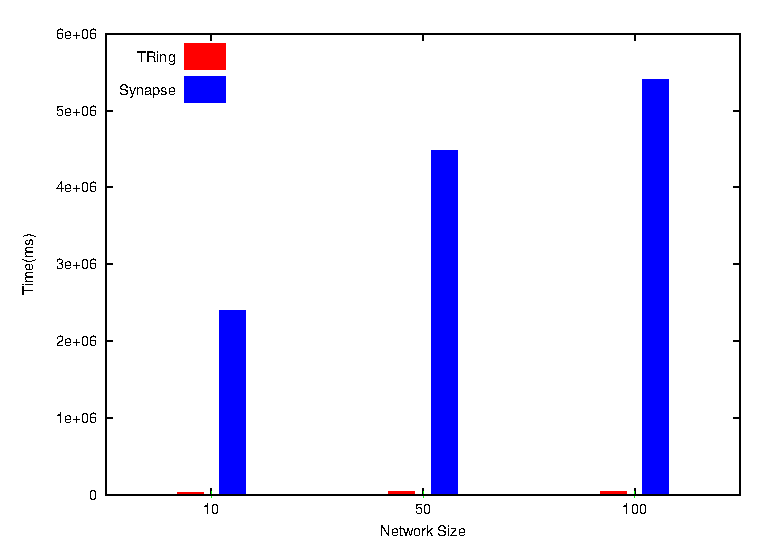
\includegraphics[width=14cm]{./images/compare_retrieve_rtt50.eps}
%\begin{center}
%  \begin{tabular}{|c||c|c|c|} \hline
%  \backslashbox{}{} & NS=10 & NS=50 & NS=100  \\ \hline \hline
%       T-Ring & 25730 ms & 46740 ms & 45068 ms  \\ \hline
%       Synapse & 2392797  ms & 4477108 ms & 5406327 ms \\ \hline
%  \end{tabular}
%\end{center}
%\caption{取得:RTT=50}
% \label{fig:compare_retrieve_rtt50}
% \end{minipage}
%\end{figure}

%\begin{figure}[htbp]
%\begin{minipage}{1\textwidth}
%    \centering
%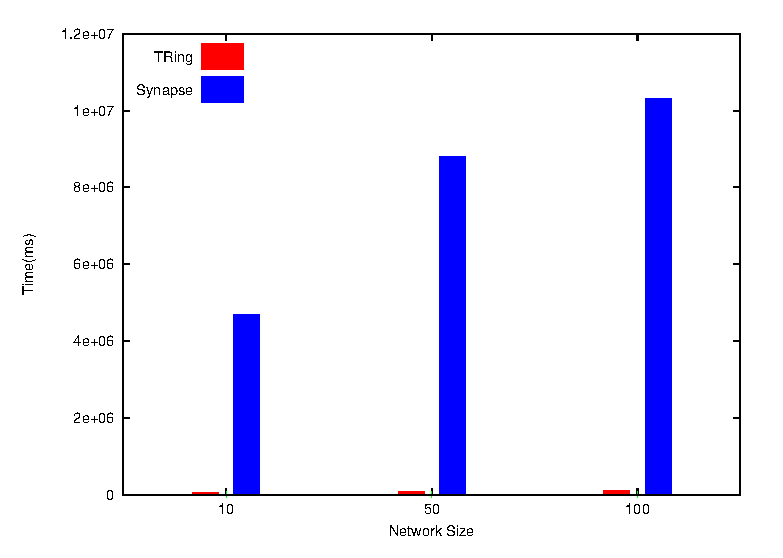
\includegraphics[width=14cm]{./images/compare_retrieve_rtt100.eps}
%\begin{center}
%  \begin{tabular}{|c||c|c|c|} \hline
%  \backslashbox{}{} & NS=10 & NS=50 & NS=100  \\ \hline \hline
%       T-Ring & 51478 ms & 90249 ms & 104476 ms  \\ \hline
%       Synapse & 4691619  ms & 8816386 ms & 10322459 ms \\ \hline
%  \end{tabular}
%\end{center}
%\caption{取得:RTT=100}
% \label{fig:compare_retrieve_rtt100}
% \end{minipage}
%\end{figure}

\section{考察}
本節では,保存ピア探索の計算コスト,保存,取得それぞれの実験の結果に関しての考察を行う.
\subsection{保存ピア探索の計算コストにおける考察}
Synapseでは,保存される全てのデータに対して保存ピアの計算が行われる.つまり,ネットワークサイズ=N,データの数=D,ホップ数=Hとすると理論値では,
\begin{equation}
H=D\cdot\log{2}N \label{1}
\end{equation}
となる.(\ref{1})における$\log{2}N$は,Chordの平均探索ホップ数である.それに対してT-Ringでは,Synapseでの所与の変数に加え,chunkの時間=C,SPの時間=S,保存されるデータの時間間隔=IT,保存されるデータの総時間=ATと,時間的な変数を加えて考えると,理論値は,
\begin{equation}
D= \frac{AT}{IT} \label{2}
\end{equation}
\begin{equation}
H=\frac{AT}{C}- \frac{AT}{S} + \frac{AT}{S} \cdot\log{2}N \label{3}
\end{equation}
となり,(\ref{2})(\ref{3})から,ATを消去すると,
\begin{equation}
H=\frac{IT \cdot D\{S - C (1- \log{2}N ) \} }{C \cdot S} \label{4}
\end{equation}
(\ref{4})となる.
(\ref{1})(\ref{4})から,SynapseとT-Ringにおけるホップ数(それぞれSynapseH,T-RingH)の割合を計算すると,
\begin{equation}
\frac{SynapseH}{TRingH}=\frac{1}{IT} \cdot \frac{S \cdot C \cdot \log{2}N }{S + C(\log{2}N -1)}     \label{5}
\end{equation}
ここから,chunkとSPの関係性について考えると,
\begin{equation}
C \cdot S \cdot \log{2}N - S + C(\log{2}N - 1) = C \cdot \log{2} N \cdot (S+1) - ( S + C )
\end{equation}
と$C>S>0$,$N>0$から,SPの値が大きくなる場合,chunkの値がSPの値に近づく場合,(\ref{5})の値が大きくなる.また,同様にITの値が小さくなるほど,(\ref{5})の値が大きくなる.

ここから,実験結果を考察すると,実験結果は,理論値とほぼ相違ないことが分かる.よって,今回はchunk,SP,データの保存間隔を以上で述べた通りに行ったが,chunk=999,SP=1000,データの保存間隔=1にした場合,Synapseのホップ数に限りなく近づく.

この保存ピア探索の計算コストは,データの保存,取得に大きく関係する.次節からこの関係性について考察する.
\subsection{データ保存における考察}
前節において,保存ピア探索の計算コストについての考察を行ったが,SynapseとT-Ringのデータの保存にかかる時間の割合は,ネットワークレイテンシ(RTT)=RTTとすると,
\begin{equation}
\frac{SynapseH}{TRingH} \cdot RTT \cdot D \label{6}
\end{equation}
となる,SynapseとT-Ringを比較した際,RTTとDは同一の環境で実験をした場合,値の違いはないので,$\frac{SynapseH}{TRingH}$において,取得時間は決定する.ここから,実験結果を考察すると,T-Ringにおける取得時間が理論値以上であることが伺える.これは,センサデータの保存を行う前段階のセンサ情報の取得による影響であると考えられる.本システムでは,センサデータがセンサノードから保存ピアに送られた際,そのセンサデータの時間とそのセンサノードの設置時間から,対象のデータの保存先が次の保存ピアに移行するのか,移行する際,異なるマスターノードに移行するのかを計算する.この計算に時間を要する分,T-Ringが理論値と異なっていると考えられる.

\subsection{データの取得における考察}
データの取得においても,保存時と同様に考え,クエリの検索範囲の半径=Rとすると,SynapseとT-Ringのデータの保存にかかる時間の割合は,
\begin{equation}
\frac{SynapseH}{TRingH} \cdot RTT \cdot D \cdot  \pi r^{2}  \label{7}
\end{equation}
となる.保存時と比較すると,対象範囲内の全ての座標を計算するため,$\pi r^{2}$倍の差が発生することとなる.このことが,実験結果において,SynapseとT-Ringの時間の差が発生した論拠であると考えられる.

\section{まとめ}
本章では,まず,本研究に評価方針,実験環境を述べた.次に,実験環境内における実験への影響を調査するため,それぞれのリージョンからICMPにおける,Message Requestを送信し,リプライが返されるまでの時間(RTT)を計測した.その結果,RTTは0.400ms以内であり,十分に無視できることを述べた.次いで,保存ピア探索における計算コスト,データの保存に要する時間,データの取得に要する時間の観点から評価を行った.その結果から,考察を行い,理論値と実際の値に齟齬が存在することを明らかにし,その違いは,T-Ringにおいて,保存や取得の対象となるデータの時間情報の取得を行う際に要する時間により生じていることに言及した.

\chapter{結論}
\begin{large}
\begin{quote}
本章では,T-Ringシステムの結論を述べる.
\end{quote}
\end{large}
\clearpage

\section{今後の課題と展望}
本研究では,センサデータの時間的特殊性に着目することにより,保存ピア探索における計算コスト,データ保存に要する時間,データ取得に要する時間について,既存の手法と比較し,それぞれ良い知見が得られた.しかし,データの取得に要する時間に関しては,依然として,課題が残る.既存手法との比較では,時間短縮に成功したが,半径10の領域から100個のデータの取得を行うに際し,時間数万msの時間を要している.想定するシナリオに挙げたように,ユーザがスマートフォンから情報を取得し,リアルタイムにアプリケーションに反映させることを斟酌すると,この所要時間では到底満足できない.よって,今後は,このデータの取得に着目した研究が必要となる.これに関する指針として,センサデータ管理のマルチレイヤ化がある.現行のT-Ringシステムは,全てのデータを生データのまま保存している.しかし,現実に取得されるデータは,10:00,11:00など切りの良い時間から取得される可能性が高いと考え得る.また,値の平均や最大,最小などが利用されるケースも存在する.このように,個々のセンサデータについての特徴は存在しないながらも,ある一定のデータが集約されることにより,特定の意味を有する1つのデータになることは十分に考えられる.これらの,データの集約による特徴ごとに,マルチレイヤで管理することにより,ユーザのクエリに対する対象データ数の削減に寄与すると考えられる.

また,本研究のメインフォーカスとして挙げてはいないが,近年,Cyber-Physical Systemsと呼ばれる,実空間情報を情報空間に取り込むことにより,新たな価値を提供することを目指す研究分野が注目されている.Cyber-Physical Systemsでは,人間や物の行動や動きを逐次記録する手法が用いられることがある.この記録データは,センサデータと同様に時間に伴って増大する.T-Ringはこのようなデータを管理する手法としても用いることが可能である.

\section{本論文のまとめ}
本研究は,従来の多次元データ管理手法がセンサデータにおける時間のような,パラメータに特徴のあるデータを対象とした手法が存在しないことに着目した.次いで,センサデータの時間的特殊性に着目したT-Ringシステムの提案を行った.このシステムの評価を行った結果,既存のシステムと比べ,データ保存,取得において,高速化を実現した.しかし,データの取得に関しては,リアルタイムアプリケーションに利用するに耐えうる所要時間ではないので,最終章において,今後の課題として取り組むべきであることに言及した.


\chapter*{謝辞}
本論文の執筆にあたり,親身になって丁寧にご指導して頂きました,慶應義塾大学環境情報学部教授徳田英幸博士に深く感謝致します.また,また,貴重なご助言を頂きました應義塾大学環境情報学部准教授高汐一紀博士,慶応義塾大学環境情報学部専任講師中澤仁博士,慶応義塾大学環境情報学部米澤拓郎特任助教,慶応義塾大学政策・メディア研究科伊藤友隆氏に深く感謝致します.

慶應義塾大学徳田研究室の諸先輩方には折に触れ貴重なご助言を頂き,また多くの議論の時間を割いて頂きました.特に,政策・メディア研究科博士課程生天目直哉氏には,本研究に対し,多くの時間を割いて頂きました.ここに多大なる感謝と尊敬の意を表します.

また,数少ない同学年として,研究活動に切磋琢磨した,伊藤瑛氏,小鷲麻奈美氏,グエンミンザン氏,KMSF,Link研究グループにおいて,研究活動だけではなく,公私に関わらず,親しく接していただいただいた井村和博氏,鈴木幸大氏,皆川昇子氏,高木慎介氏,宇佐美真之介氏,豊田智也氏,荻野メリッサ氏を始めとした諸先輩,後輩方,研究で疲弊している中,いつも強引に徹夜でのサッカーゲームに誘ってくれて,疲れを増幅させながらも精神衛生を整え続けてくれた二神直也氏,阿部寛氏に深く感謝し,謝辞と致します.

%%%%%%%%%%%%%%%%%%%%%%%%%%%%%%%%%%%%%%%%%%%%%%%%%%%%%%%%%%%%%%%%%%%%%%%%%%%%%%%%
%本研究の機会を与えてくださり,絶えず丁寧なご指導を賜りました,慶應義塾大学環境情報学部教授徳田英幸博士に深く感謝致します.また,貴重なご助言を頂きました應義塾大学環境情報学部准教授高汐一紀博士に深く感謝致します.
%また,慶應義塾大学徳田研究室の諸先輩方には折に触れ貴重なご助言を頂き,また多くの議論の時間を割いて頂きました.特に政策メディア研究科修士課程小川正幹氏,今枝卓也氏には,本論文の執筆にあたってご指導を頂きました.また政策メディア研究科講師中澤仁博士には本研究を進めるにあたって多くの励ましとご指導を頂きました.ここに深い感謝の意を表します.
%最後に,研究生活を経済的にだけでなく,精神的にも支えてくれた家族,研究の日々を家族同然に同じ時間を共に過ごした慶應義塾大学総合政策学部4年天野雅哉氏,慶應義塾大学環境情報学部4年米川賢治氏,モヒカンの頃が懐かしい井村和博氏,日本,研究の日々を共に過ごしたACE 研究グループの勝治宏基氏,その他多くの友人に深く感謝し,謝辞と致します.
\begin{flushright}
\today\\
寺山淳基
\end{flushright}

\bibliographystyle{junsrt}
\bibliography{ref}


\appendix
%\input{bayes.tex}
%\input{appendix.tex}
%\input{appendix2.tex}
%\input{appendix3.tex}

\end{document}
